% MedVision Q1 manuscript master file for Informatics and Health.

\documentclass[a4paper,fleqn]{cas-sc}

\usepackage{amsmath,amssymb}
\usepackage{booktabs}
\usepackage{float}
\usepackage{graphicx}
\usepackage{multirow}
\usepackage{natbib}
\usepackage{xcolor}
\usepackage{hyperref}
\hypersetup{hypertexnames=false,hidelinks}

\graphicspath{{figures/}}

% Use a clean manuscript page style: suppress the CAS template's default
% running title and the "Preprint submitted to Elsevier" footer while
% retaining unobtrusive page numbering.
\ExplSyntaxOn
\cs_set:Npn \__first_footerline: {}
\cs_set:Npn \__first_head: {}
\cs_set:Npn \__cas_head: {}
\ExplSyntaxOff
% No ORCID identifiers were supplied; suppress the template's empty ORCID footnote.
\RenewDocumentCommand \printorcid { } { }
\pagestyle{cas}

\begin{document}

\title[mode=title]{Quantifying Modality Inertia in Medical Vision-Language Models: Image Contribution Metric, Gate Stagnation, and the Failure of Debiasing Under Label Circularity}

\author{Nafis Al Rahman}
\author{Tanvir Mahmud}

\begin{abstract}
Background. Medical vision--language models can report high accuracy while
relying on report text rather than radiographic evidence. This risk is
especially difficult to interpret in MIMIC-CXR, where CheXpert targets are
generated from the same reports that may remain available as model inputs. We
evaluated whether text-debiasing increases incremental image information or
merely changes aggregate performance.

Methods. We audited a three-class MIMIC-CXR-derived classifier comprising
Normal, Pneumonia, and Pneumothorax across eight random seeds and five
conditions: baseline gated fusion, a learned text-prior product-of-experts
variant, a noise-sensitivity variant, an exploratory grounding-aware variant,
and an adaptive-gate variant. Each condition used 455 held-out studies;
report-preserving Gray-Square replacement, text-only, and image-only controls
were retained. The primary endpoint was the Image Contribution Metric (ICM),
with a pre-specified equivalence interval of minus 0.01 to plus 0.01. We
combined paired seed-level inference with calibration, gate extraction, and
qualitative saliency checks.

Findings. Baseline Macro-F1 was 0.9397 plus or minus 0.0061, compared with
0.9381 for the retained Gray-Square control. Baseline ICM was 0.0016 plus or
minus 0.0065; the signed-rank test was non-significant (p = 0.4219), while two
one-sided tests supported equivalence to zero within the operational interval
(p = 0.0040). No text-debiasing condition demonstrated a robust increase in
ICM. The text-prior variant increased expected calibration error from 0.0237
to 0.0621 and Brier score from 0.0522 to 0.0685. Extracted baseline gates
remained near initialization, with an overall mean of 0.49975.

Interpretation. On this report-linked benchmark, near-ceiling performance was
compatible with a report shortcut and did not establish incremental image
grounding. The result is a diagnostic warning about label--report circularity
and endpoint design, not evidence that radiographs are universally unnecessary.
Independent labels, corrected implementations, matched controls, provenance
manifests, and external cohorts are required before making broader clinical
claims.
\end{abstract}

\begin{keywords}
medical vision--language model \sep modality inertia \sep gate stagnation
\sep Image Contribution Metric \sep label circularity \sep MIMIC-CXR
\end{keywords}

\begingroup
\sloppy
\maketitle
\endgroup

% MedVision manuscript -- Introduction section

\section{Introduction}\label{sec:introduction}

Medical vision--language models (VLMs) combine radiographs with the clinical reports
that accompany them. This pairing is valuable because images encode visual
structure whereas reports provide findings and context; resources such as
MIMIC-CXR make both modalities available at scale \citep{johnson2019mimiccxr}.
High multimodal accuracy, however, does not establish that the model used
clinically meaningful visual evidence. A model may exploit a report shortcut or
another predictive feature that is easier to optimise than image information.

This distinction is especially important when targets are report-derived. The
CheXpert labeler converts report language into uncertainty-aware
chest-radiograph labels \citep{irvin2019chexpert}. If the same report, or its
\texttt{findings} field, is also supplied to the model, the target and one
input modality share an information source. The resulting task may reward
linguistic recognition of the report-derived label rather than independent
image-grounded recognition. Report-conditioned prediction can still be useful;
the problem is claiming incremental image evidence from aggregate accuracy
alone.

Recent evidence shows why this distinction matters in medical VLM evaluation.
Performance can change with the amount of clinical context supplied before an
image is seen, and apparently correct multimodal answers may be accompanied by
unreliable visual rationales \citep{wang2026clinicalcontext,jin2024hiddenflaws}.
Large-scale chest-radiography audits have likewise found that removing the
image can leave performance largely intact, while consistency across prompts
can coexist with non-visual decision making \citep{lotfinia2026needimage,sadanandan2026consistentdangerous}.
Counterfactual prototype methods can improve interpretability, but they do not
replace a report-preserving intervention that directly measures the change in
the prediction \citep{chiang2026cxrnexus}.

Conventional model comparisons rarely replace the image while holding the
report, label, architecture, and evaluation protocol fixed. Similarly, a
non-zero fusion gate or attention map is not necessarily causal evidence of
visual use: gates can remain near initialization and a one-token interaction
cannot show word--region alignment. Text-debiasing methods may therefore lower
a score without creating an independent visual signal when the endpoint itself
is linked to text.

We present a controlled audit of a three-class MIMIC-CXR-derived task
(Normal, Pneumonia, and Pneumothorax). The model receives a frontal radiograph
and the report's \texttt{findings} field. We compare full multimodal models
with a report-preserving Gray-Square control that replaces every radiograph by
a constant tensor, together with text-only and image-only controls. Four
fusion or text-debiasing variants are evaluated alongside the project's
baseline gated dual-path model (CADQ). We
report discrimination, calibration, class-specific behaviour, learned image
gates, and qualitative gradient-weighted class activation mapping (Grad-CAM)
checks. The primary diagnostic is the Image
Contribution Metric (ICM), defined as the relative Macro-F1 difference between
the full model and the Gray-Square reference; paired inference is performed at
the trained-seed level because held-out studies recur across seeds.

The audit asks whether removing image information changes performance, whether
the interventions increase incremental image contribution, whether checkpoint
gates show learned reliance or stagnation, and whether calibration and
class-specific results qualify the headline metrics. It contributes a
report-preserving image ablation, seed-level uncertainty and calibration
reporting, and an explicit analysis of label provenance and control asymmetry.
The study is a diagnostic evaluation, not a new clinical predictor or a claim
that radiographs are generally unnecessary. Its interpretation is limited to
this report-linked cohort, preprocessing path, and checkpoint archive; broader
claims require corrected implementations, independent labels, matched controls,
and external validation. Reporting follows the transparency principles of the
Checklist for Artificial Intelligence in Medical Imaging (CLAIM) and the
TRIPOD+AI framework \citep{mongan2024claim,collins2024tripodai}.

% MedVision manuscript -- Related Work section

\section{Related Work}\label{sec:related-work}

\subsection{Medical image--text learning and report-derived targets}
Paired image--report resources support contrastive and local alignment methods
such as ConVIRT and GLoRIA, while clinical-domain language models improve the
handling of negation and uncertainty \citep{zhang2022convirt,huang2021gloria,boecking2022textsemantics}.
These methods establish the value of reports but do not show that a downstream
prediction depends on the image. MIMIC-CXR links radiographs to free-text
reports, whereas CheXpert derives uncertainty-aware labels from report language
\citep{johnson2019mimiccxr,irvin2019chexpert}. Report-labeling tools can also
propagate errors and subgroup differences \citep{sabottke2024targetselection,santomartino2024nlplabeling}.
The present audit therefore distinguishes report-conditioned prediction from
independent image-grounded diagnosis when both target and text input share a
report source.

\subsection{Shortcut learning and unimodal bias}
Shortcut-learning research shows that high in-distribution accuracy can arise from
predictive but unintended features \citep{geirhos2020shortcut}. In radiology,
acquisition devices, population structure, annotation practice, and clinical
context can create such shortcuts \citep{gichoya2023shortcuts}. In visual
question answering, VQA-CP, GVQA, product-of-experts methods, and RUBi reduce
answer or language priors by encouraging visual evidence \citep{agrawal2018dontassume,clark2019easyway,cadene2019rubi}.
They motivate LMH-style debiasing, but do not resolve the harder case in which
the benchmark label is itself text-derived.

\subsection{Auditing modality reliance}
Recent multimodal evaluations separate correctness from evidence dependence:
correct answers can be accompanied by flawed visual rationales, and stable
predictions need not be image-reliant \citep{jin2024hiddenflaws,sadanandan2026consistentdangerous}.
Chest-X-ray studies further report heterogeneity after controlling for clinical
context \citep{wang2026clinicalcontext}. Causal audits using image occlusion,
cross-patient replacement, and text-only comparisons provide a direct precedent
for testing image use \citep{lotfinia2026needimage}. Prototype and counterfactual
methods can improve saliency, but heatmaps alone cannot establish that image
removal changes a decision \citep{chiang2026cxrnexus}.

\subsection{Fusion gates and explanation limits}
Gated multimodal units learn modality weights, yet a non-zero or balanced gate
is not causal attribution \citep{arevalo2017gmu}. A gate may remain near its
initialization when the objective does not identify a different value. Likewise,
reasoning traces or plausible radiologist-style explanations are useful
interfaces but not grounding tests \citep{myronenko2025reasoningcxr}. The
present study combines checkpoint gate extraction with a report-preserving
image intervention and treats Grad-CAM as a qualitative sanity check.

\subsection{Positioning of the present study}
Prior work treats image--text learning, report-label uncertainty, shortcut bias,
and behavioural audits separately. We examine their intersection using
report-preserving, text-only, and image-only controls, an operational ICM,
checkpoint gates, and seed-level inference. The study tests incremental visual
evidence without claiming that report-conditioned prediction or all medical
VLMs are invalid.

% MedVision manuscript -- Methods section
% Citation keys are defined in methodology_references.bib.

\section{Methods}\label{sec:methods}

\subsection{Study design and analysis scope}\label{sec:study-design}
We conducted a controlled audit of a medical vision--language classifier. The
estimand was the incremental image contribution when the report remained
available. The principal intervention replaced each radiograph with a uniform
gray tensor while retaining the text, label, architecture, and evaluation
protocol. Full multimodal predictions were compared with this control and with
text-only and image-only models.

The replication unit for confirmatory inference was a trained model at a fixed
seed. Eight seeds (42, 123, 456, 789, 1010, 1111, 1212, 1313) were used for
baseline CADQ, the LearnedMixinFusion text-prior variant (LMH),
Noise-Consistency, and Adaptive-CADQ. The exploratory grounding-aware variant
(GACR-B) was added after the initial plan. Because the same test studies recur
across seeds, subjects were not treated as independent observations across
seeds. ICM was the primary diagnostic; calibration and gate behaviour were
secondary outcomes. The Adaptive-CADQ extension and GACR-B are labelled
post hoc.

Figure~\ref{fig:cohort-flow} records the complete cohort-construction path and
the patient-level analysis split. Figure~\ref{fig:method-workflow} summarizes
the corresponding audit workflow from data provenance through paired inference.

\begin{figure}[pos=htbp]
\centering
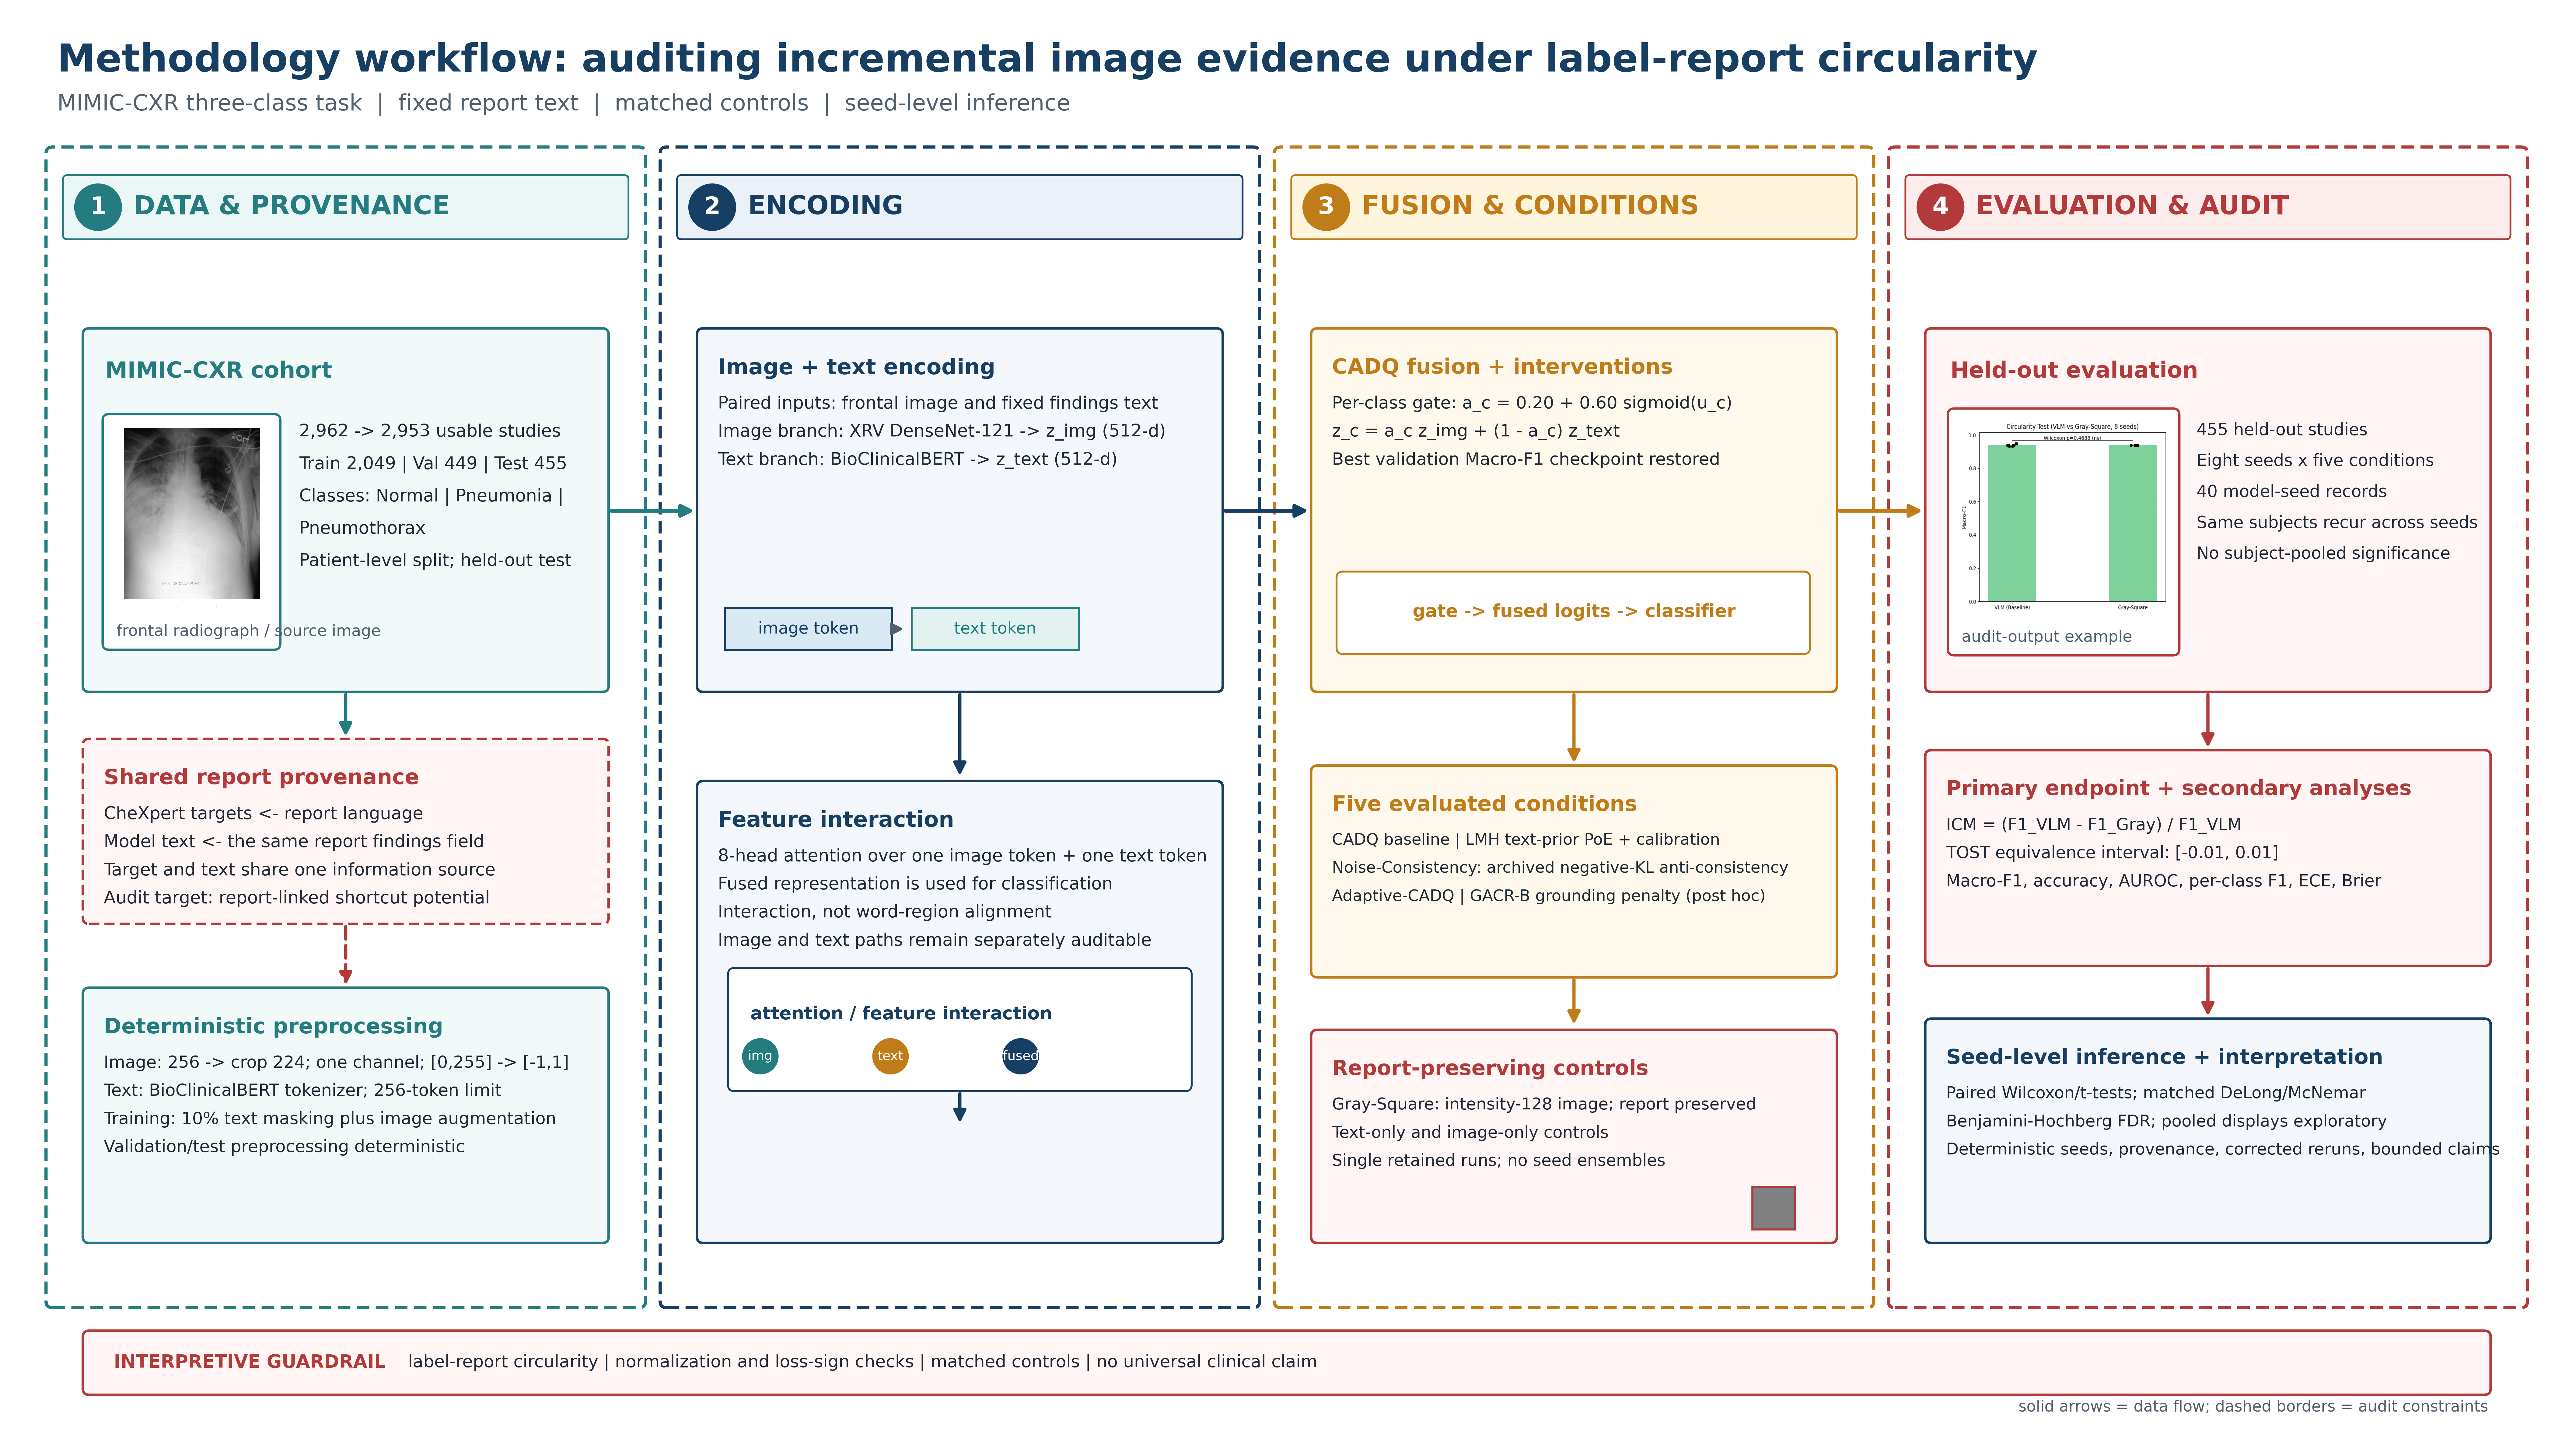
\includegraphics[width=\linewidth]{figures/methodology_audit_workflow_visual_v2.png}
\caption{Audit workflow from MIMIC-CXR data provenance and patient-level splitting
through image/text encoding, CADQ fusion, report-preserving controls, and
seed-level paired inference.}
\label{fig:method-workflow}
\end{figure}

\begin{figure}[pos=htbp]
\centering
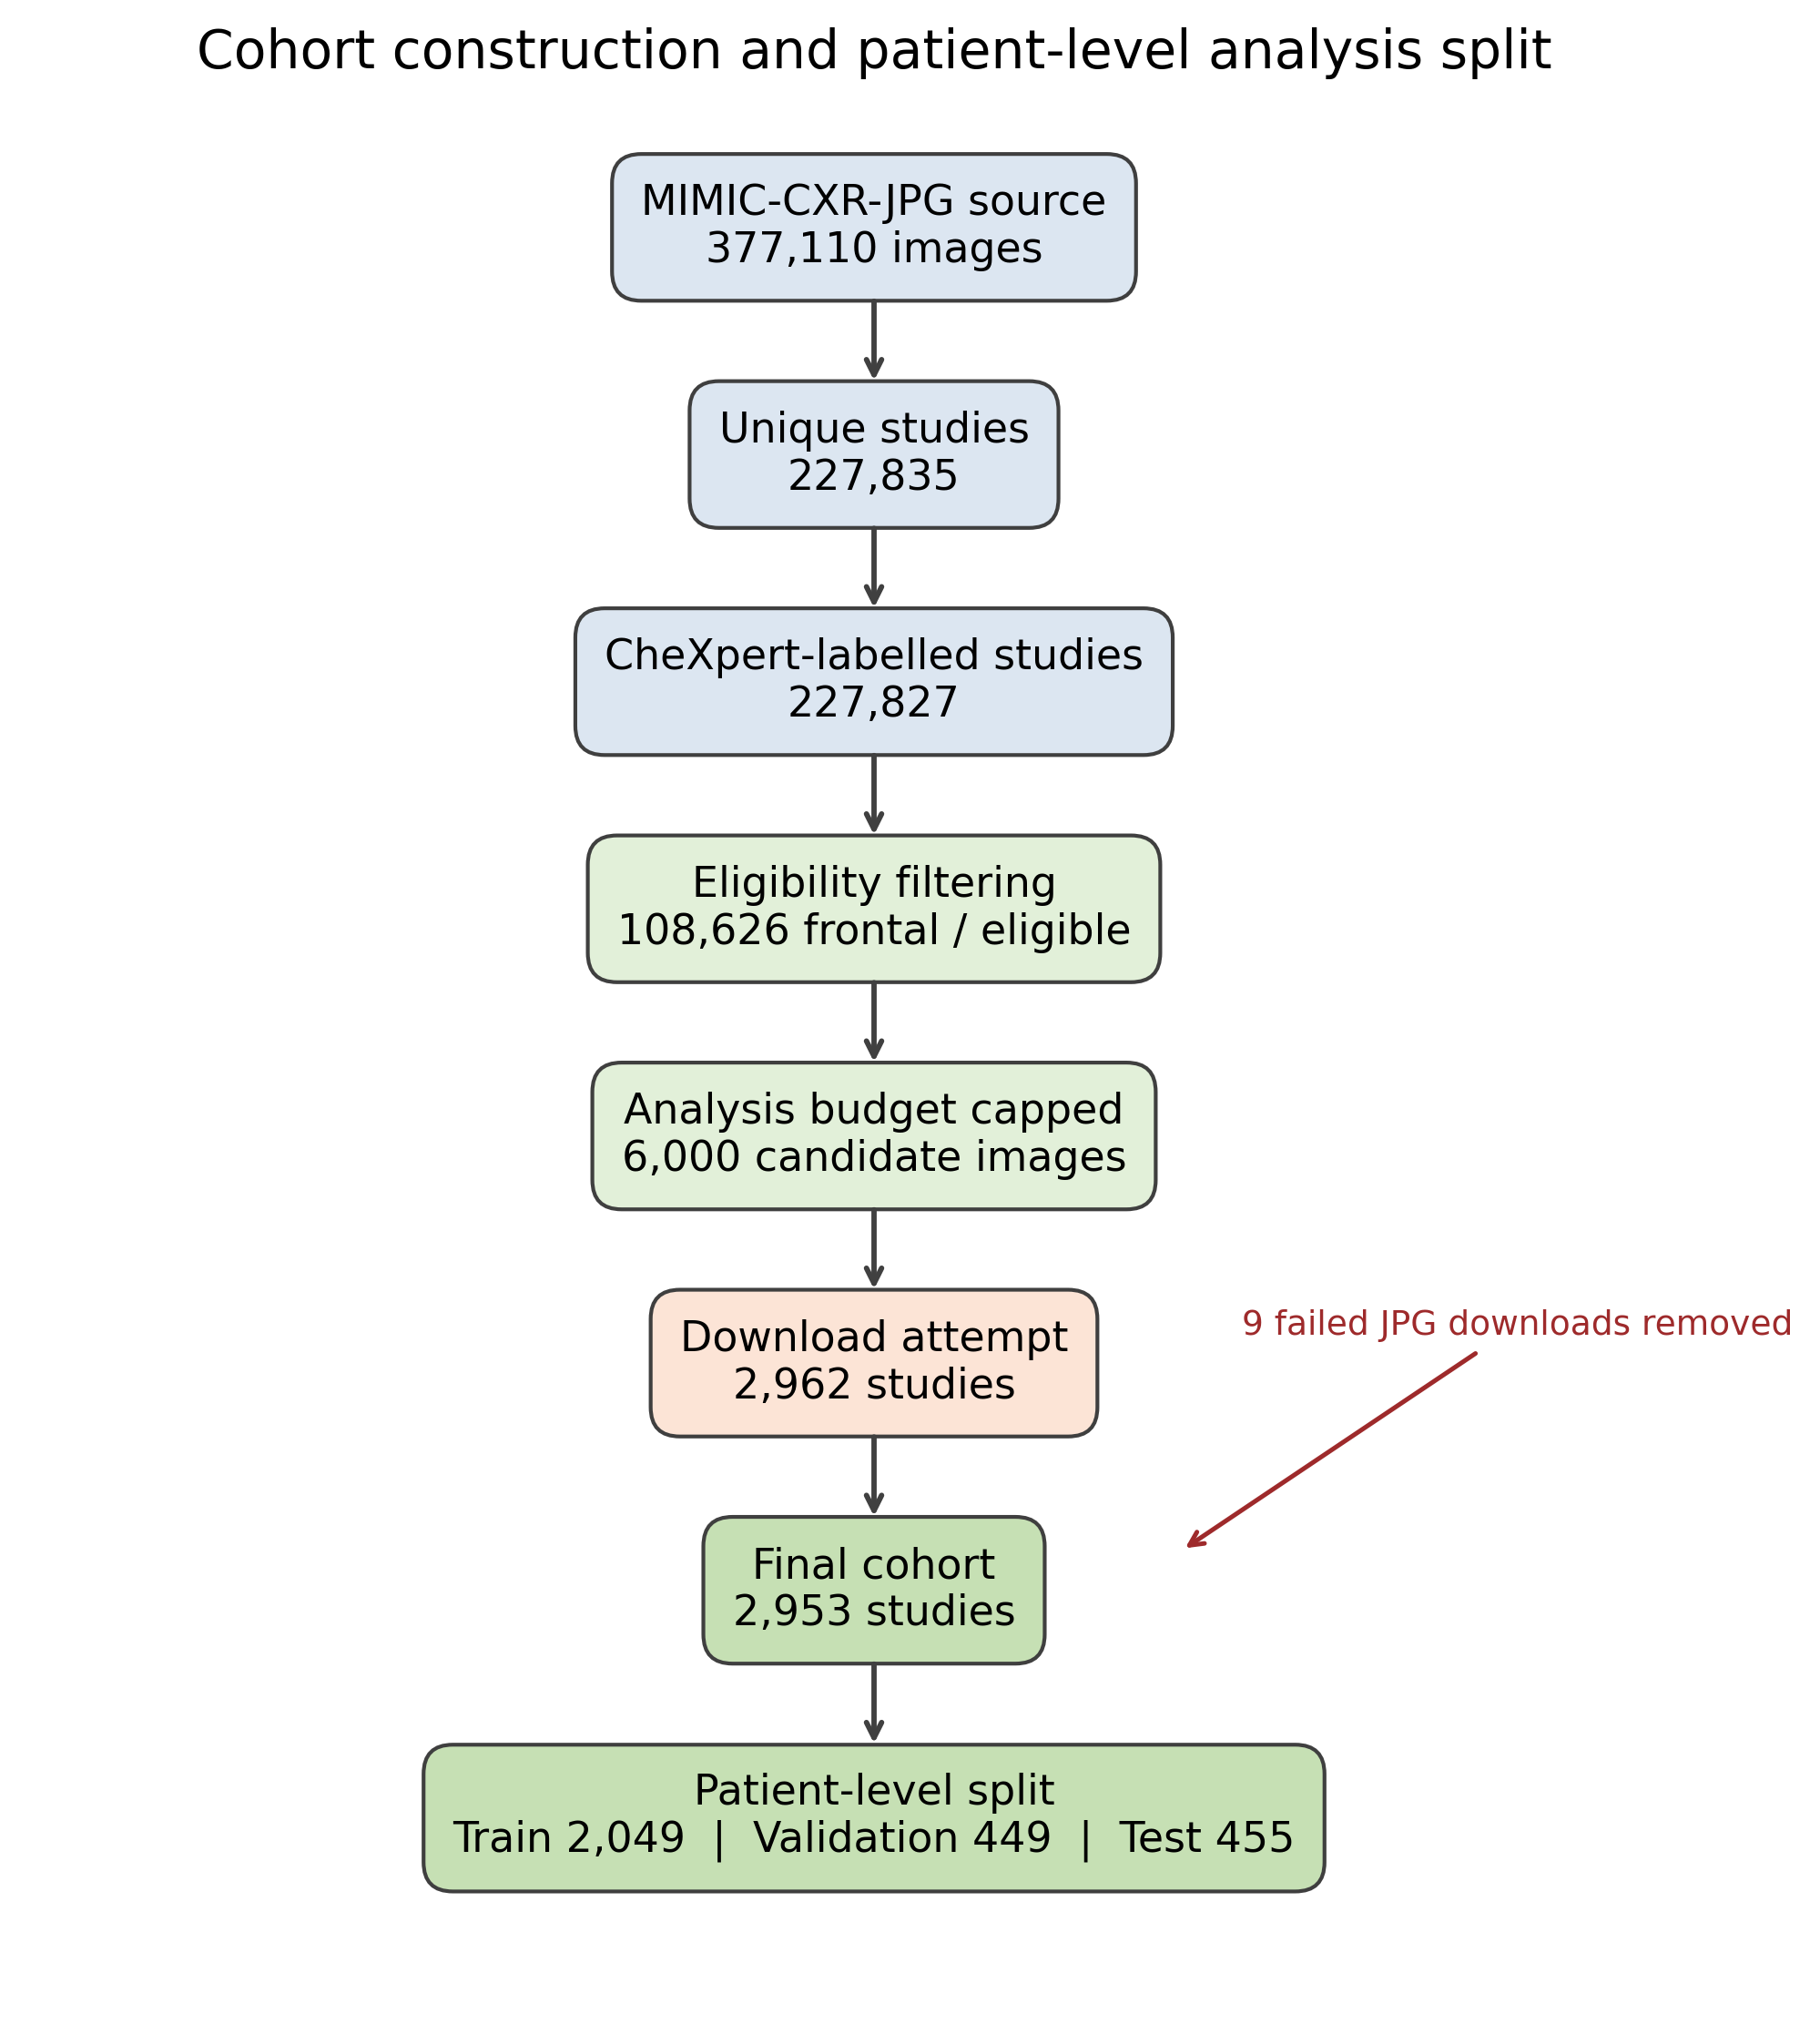
\includegraphics[width=0.52\linewidth]{figures/cohort_flow.png}
\caption{Cohort construction and patient-level analysis split. Nine failed JPG
downloads were removed before the final 2,953-study cohort was partitioned.}
\label{fig:cohort-flow}
\end{figure}

\subsection{Data source and cohort construction}\label{sec:data-cohort}
MIMIC-CXR JPG images and reports were accessed through PhysioNet credentialing
and the applicable Data Use Agreement \citep{johnson2019mimiccxr}. From 2,962
candidate records, nine missing JPG files were removed, leaving 2,953 studies
(2,049 training, 449 validation, and 455 test). Only frontal radiographs were
retained. The three classes were Normal, Pneumonia, and Pneumothorax; class
caps were 2,500, 2,500, and 1,000, respectively. The inherited patient-level
split contained no subject overlap and 47 Pneumothorax studies in the test set.
For transparency, the source-to-analysis flow was 377,110 JPG images, 227,835
unique studies, 227,827 CheXpert-labelled studies, 108,626 eligible frontal
studies, a 6,000-candidate analysis cap, 2,962 download attempts, and 2,953
retained studies after the nine download failures (Fig.~\ref{fig:cohort-flow}).

CheXpert generated the targets from report language using the project’s
uncertain-to-negative mapping \citep{irvin2019chexpert}. The model received the
same report’s \texttt{findings} field. Thus, the experiment audits
label--report circularity rather than an independent image-only diagnostic
task. This secondary analysis used de-identified data; no participants were
recruited and no direct identifiers were accessed. MIMIC-CXR was released for
credentialed research under the source-study IRB approvals; no additional
local participant recruitment or intervention was undertaken for this audit.

\subsection{Preprocessing}\label{sec:preprocessing}
Findings text was tokenized with the
\texttt{emilyalsentzer/Bio\_ClinicalBERT} tokenizer and truncated or padded to
256 tokens. During training, 10\% of strings were replaced by an empty string;
validation and test text was unmasked. Images were resized to $256\times256$,
randomly cropped to $224\times224$, converted to one channel, and mapped from
$[0,255]$ to $[-1,1]$. Training used horizontal flips, rotation (up to
$10^{\circ}$), translation (5\%), and brightness/contrast jitter (0.2); the
class-aware minority transform increased rotation to $15^{\circ}$ and used
translation up to 10\%, scale 0.9--1.1, shear up to $10^{\circ}$, stronger
jitter (0.3), and Gaussian blur. Validation and test images were deterministically
resized and mapped. The archived $[-1,1]$ mapping may not match the native
TorchXRayVision convention and requires a corrected rerun
\citep{cohen2022torchxrayvision}.

\subsection{Model architecture}\label{sec:architecture}
The image branch used TorchXRayVision (XRV) DenseNet-121 with
\texttt{densenet121-res224-mimic\_ch} weights \citep{huang2017densenet,cohen2022torchxrayvision}.
Its output was projected to 512 dimensions with linear, LayerNorm, Gaussian
Error Linear Unit (GELU), and
dropout (0.25); the convolutional stem and first dense block were frozen. The
text branch used Bio\_ClinicalBERT, with its first four layers frozen, and an
analogous 512-dimensional projection \citep{devlin2019bert,alsentzer2019clinicalbert}.
The projected image was one query token and projected text one key/value token
in an eight-head batch-first attention block with residual LayerNorm. This is a
feature interaction, not token-level word--region alignment; its single-key
attention is degenerate and is not interpreted as causal grounding.

\subsection{Fusion variants and controls}\label{sec:variants}
CADQ produced image and text logits and combined them with a learnable
per-class gate \citep{arevalo2017gmu}:
\begin{equation}
\alpha_c=0.20+0.60\operatorname{sigmoid}(u_c),\qquad
z_c=\alpha_cz^{\mathrm{img}}_c+(1-\alpha_c)z^{\mathrm{text}}_c,
\end{equation}
with $u_c=(-0.5,0,0.5)$ and initial gates approximately
$(0.4265,0.5000,0.5735)$. LMH added a five-fold out-of-fold
term-frequency/inverse-document-frequency (TF--IDF)
logistic text-prior branch (5,000 unigram/bigram features, stop-word removal,
balanced weights), validation temperature calibration, $\epsilon=0.1$
smoothing, an input-dependent prior gate, and an entropy penalty (weight 0.05,
annealed for three epochs) following the product-of-experts debiasing rationale
of Cadene et al. \citep{cadene2019rubi}. It was warm-started from CADQ.

Noise-Consistency added Gaussian image noise ($\sigma=0.25$) and the archived
term $\mathcal{L}_{NC}=-D_{KL}(p_{clean}\|p_{noisy})$ based on
Kullback--Leibler (KL) divergence to a minimised loss. It
therefore rewards divergence and is reported as anti-consistency/noise
sensitivity; a positive-KL rerun is required for a conventional consistency
claim. Adaptive-CADQ replaced the static gate with a sample-dependent scalar
from image/text entropies through a $2\rightarrow16\rightarrow1$ multilayer
perceptron (MLP). GACR-B
used an out-of-fold text baseline and a cosine penalty (weight 0.3) on examples
where that baseline was wrong; it is exploratory and follows the grounding-aware
consistency intervention of Sadanandan and Behzadan
\citep{sadanandan2026consistentdangerous}.

All controls used the same test studies. Image-only used the XRV encoder and a
512-to-256 classifier; text-only used frozen Bio\_ClinicalBERT and a
768-to-256 classifier. Gray-Square replaced each image with a constant
intensity-128 tensor while preserving the report and multimodal path. Retained
image-only and Gray-Square outputs were single runs, not seed ensembles.

\subsection{Training and checkpoint selection}\label{sec:training}
Models were trained for 10 epochs with AdamW \citep{loshchilov2019adamw}, differential learning rates of
$10^{-5}$ for image/text backbones, $10^{-4}$ for fusion and LMH heads, and
$5\times10^{-5}$ for static gates; weight decay was $10^{-4}$. OneCycleLR used
10\% warm-up \citep{smith2019superconvergence}. Physical batch size was 8 with four accumulation steps (effective
32), mixed precision, and gradient scaling. Training used focal
cross-entropy ($\gamma=1.5$), label smoothing 0.05, and effective-number
weights ($\beta=0.99$) \citep{lin2017focalloss}; class-aware sampling replicated
Pneumothorax up to fivefold and Pneumonia up to threefold. The best validation
Macro-F1 checkpoint was restored for multimodal variants. The archived
image-only control did not consistently restore its best state and is
descriptive.

\subsection{Endpoints and statistical analysis}\label{sec:statistics}
The primary endpoint was
\begin{equation}
\mathrm{ICM}=\frac{F1_{VLM}-F1_{Gray}}{F1_{VLM}},
\end{equation}
where positive values indicate an incremental gain from the real image. The two
one-sided tests (TOST) procedure tested equivalence to zero within
$[-0.01,0.01]$, an operational margin rather
than a clinical threshold \citep{lakens2017equivalence}. Per seed, we computed
macro-averaged F1 score (Macro-F1), per-class F1, accuracy, one-versus-rest area under the receiver
operating characteristic curve (Macro-AUROC), confusion matrices, ten-bin
expected calibration error (ECE), and multiclass Brier score. Paired Wilcoxon tests
(Pratt zero handling), paired $t$-tests, bootstrap intervals, and Cohen’s $d$
were used for matched seed differences; ECE/Brier were recomputed from retained
probability arrays and absent outputs were recorded as N/A, never zero.

DeLong AUROC comparisons for correlated curves \citep{delong1988roc} and
McNemar tests for paired classification decisions \citep{mcnemar1947correlated}
were performed within matched seeds; studies were never concatenated across
seeds for confirmatory inference. Any pooled display is exploratory.
Benjamini--Hochberg controlled false-discovery rate within each test family
\citep{benjamini1995fdr}, with two-sided $p<0.05$ nominally. Gate values were
extracted from saved checkpoint logits using the bounded equation above; manual
or hard-coded plot values were excluded.

\subsection{Reproducibility safeguards}\label{sec:reproducibility}
Python, NumPy, and PyTorch seeds were fixed and deterministic cuDNN settings
enabled. Run metadata, validation history, checkpoints, predictions,
probabilities, and configurations were saved. The fixed archive contains
duplicate merge keys without a preserved source-priority rule or hash manifest;
results are therefore tied to this snapshot and require provenance locking.
The normalisation issue, negative-KL implementation, unequal post-hoc history,
and image-only checkpoint discrepancy are reported explicitly. Reporting follows
CLAIM and TRIPOD+AI \citep{mongan2024claim,collins2024tripodai}.

% MedVision manuscript -- Results section

\section{Results}\label{sec:results}

\subsection{Analysis set and output completeness}\label{sec:results-completeness}
The fixed-merge archive contained 40 model--seed records (five conditions and
eight seeds), each evaluated on the same 455 held-out studies. Single retained
outputs were available for image-only, text-only, and Gray-Square controls.
GACR-B was post hoc and exploratory. Duplicate keys were resolved by the
first-seen archive value; because a deterministic source-priority rule and hash
manifest were not preserved, results remain tied to this snapshot. ECE and
Brier score were recomputed from probability arrays in the companion pickle
because the JSON summary omitted them. All confirmatory comparisons were paired
at seed level; repeated test studies were not concatenated across seeds.

\subsection{Predictive performance and calibration}\label{sec:results-primary}
Baseline CADQ achieved Macro-F1 $0.9397\pm0.0061$, accuracy
$0.9607\pm0.0032$, and Macro-AUROC $0.9974\pm0.0004$ (Table~\ref{tab:primary-performance}).
LMH had the highest Macro-F1 ($0.9435\pm0.0093$) but lower, more variable
AUROC ($0.9849\pm0.0113$). Noise-Consistency had the lowest confirmatory
Macro-F1 ($0.9346\pm0.0075$); Adaptive-CADQ was close to baseline. Exploratory
GACR-B reached $0.9417\pm0.0059$.

\begin{table}[pos=htbp]
\centering
\caption{Primary test-set performance across eight seeds (mean $\pm$ standard
deviation [SD]).
GACR-B was exploratory and post hoc.}
\label{tab:primary-performance}
\small
\begin{tabular}{lccc}
\toprule
Condition & Macro-F1 & Accuracy & Macro-AUROC\\
\midrule
Baseline CADQ       & 0.9397 $\pm$ 0.0061 & 0.9607 $\pm$ 0.0032 & 0.9974 $\pm$ 0.0004\\
LMH                 & 0.9435 $\pm$ 0.0093 & 0.9596 $\pm$ 0.0070 & 0.9849 $\pm$ 0.0113\\
Noise-Consistency   & 0.9346 $\pm$ 0.0075 & 0.9560 $\pm$ 0.0039 & 0.9960 $\pm$ 0.0013\\
GACR-B (exploratory)& 0.9417 $\pm$ 0.0059 & 0.9610 $\pm$ 0.0042 & 0.9972 $\pm$ 0.0005\\
Adaptive-CADQ      & 0.9388 $\pm$ 0.0072 & 0.9610 $\pm$ 0.0044 & 0.9972 $\pm$ 0.0008\\
\bottomrule
\end{tabular}
\end{table}

Baseline per-class F1 was 0.9755 for Normal, 0.9624 for Pneumonia, and 0.8810
for Pneumothorax (Table~\ref{tab:calibration-class}). LMH improved Pneumothorax
F1 to 0.9003 but reduced Pneumonia F1 to 0.9575. Noise-Consistency had the
widest Pneumothorax variation; Adaptive-CADQ had the most stable Pneumonia F1.

\begin{table}[pos=htbp]
\centering
\caption{Calibration and per-class F1 across eight seeds (mean $\pm$ SD).}
\label{tab:calibration-class}
\scriptsize
\begin{tabular}{lccccc}
\toprule
Condition & ECE & Brier & Normal F1 & Pneumonia F1 & Pneumothorax F1\\
\midrule
Baseline CADQ        & 0.0237 $\pm$ 0.0048 & 0.0522 $\pm$ 0.0040 & 0.9755 $\pm$ 0.0032 & 0.9624 $\pm$ 0.0055 & 0.8810 $\pm$ 0.0174\\
LMH                  & 0.0621 $\pm$ 0.0160 & 0.0685 $\pm$ 0.0213 & 0.9726 $\pm$ 0.0066 & 0.9575 $\pm$ 0.0077 & 0.9003 $\pm$ 0.0191\\
Noise-Consistency    & 0.0347 $\pm$ 0.0137 & 0.0655 $\pm$ 0.0130 & 0.9754 $\pm$ 0.0044 & 0.9530 $\pm$ 0.0058 & 0.8753 $\pm$ 0.0237\\
GACR-B (exploratory) & 0.0245 $\pm$ 0.0023 & 0.0540 $\pm$ 0.0038 & 0.9741 $\pm$ 0.0043 & 0.9630 $\pm$ 0.0066 & 0.8880 $\pm$ 0.0167\\
Adaptive-CADQ       & 0.0241 $\pm$ 0.0070 & 0.0527 $\pm$ 0.0028 & 0.9776 $\pm$ 0.0054 & 0.9616 $\pm$ 0.0029 & 0.8772 $\pm$ 0.0175\\
\bottomrule
\end{tabular}
\end{table}

\begin{figure}[pos=htbp]
\centering
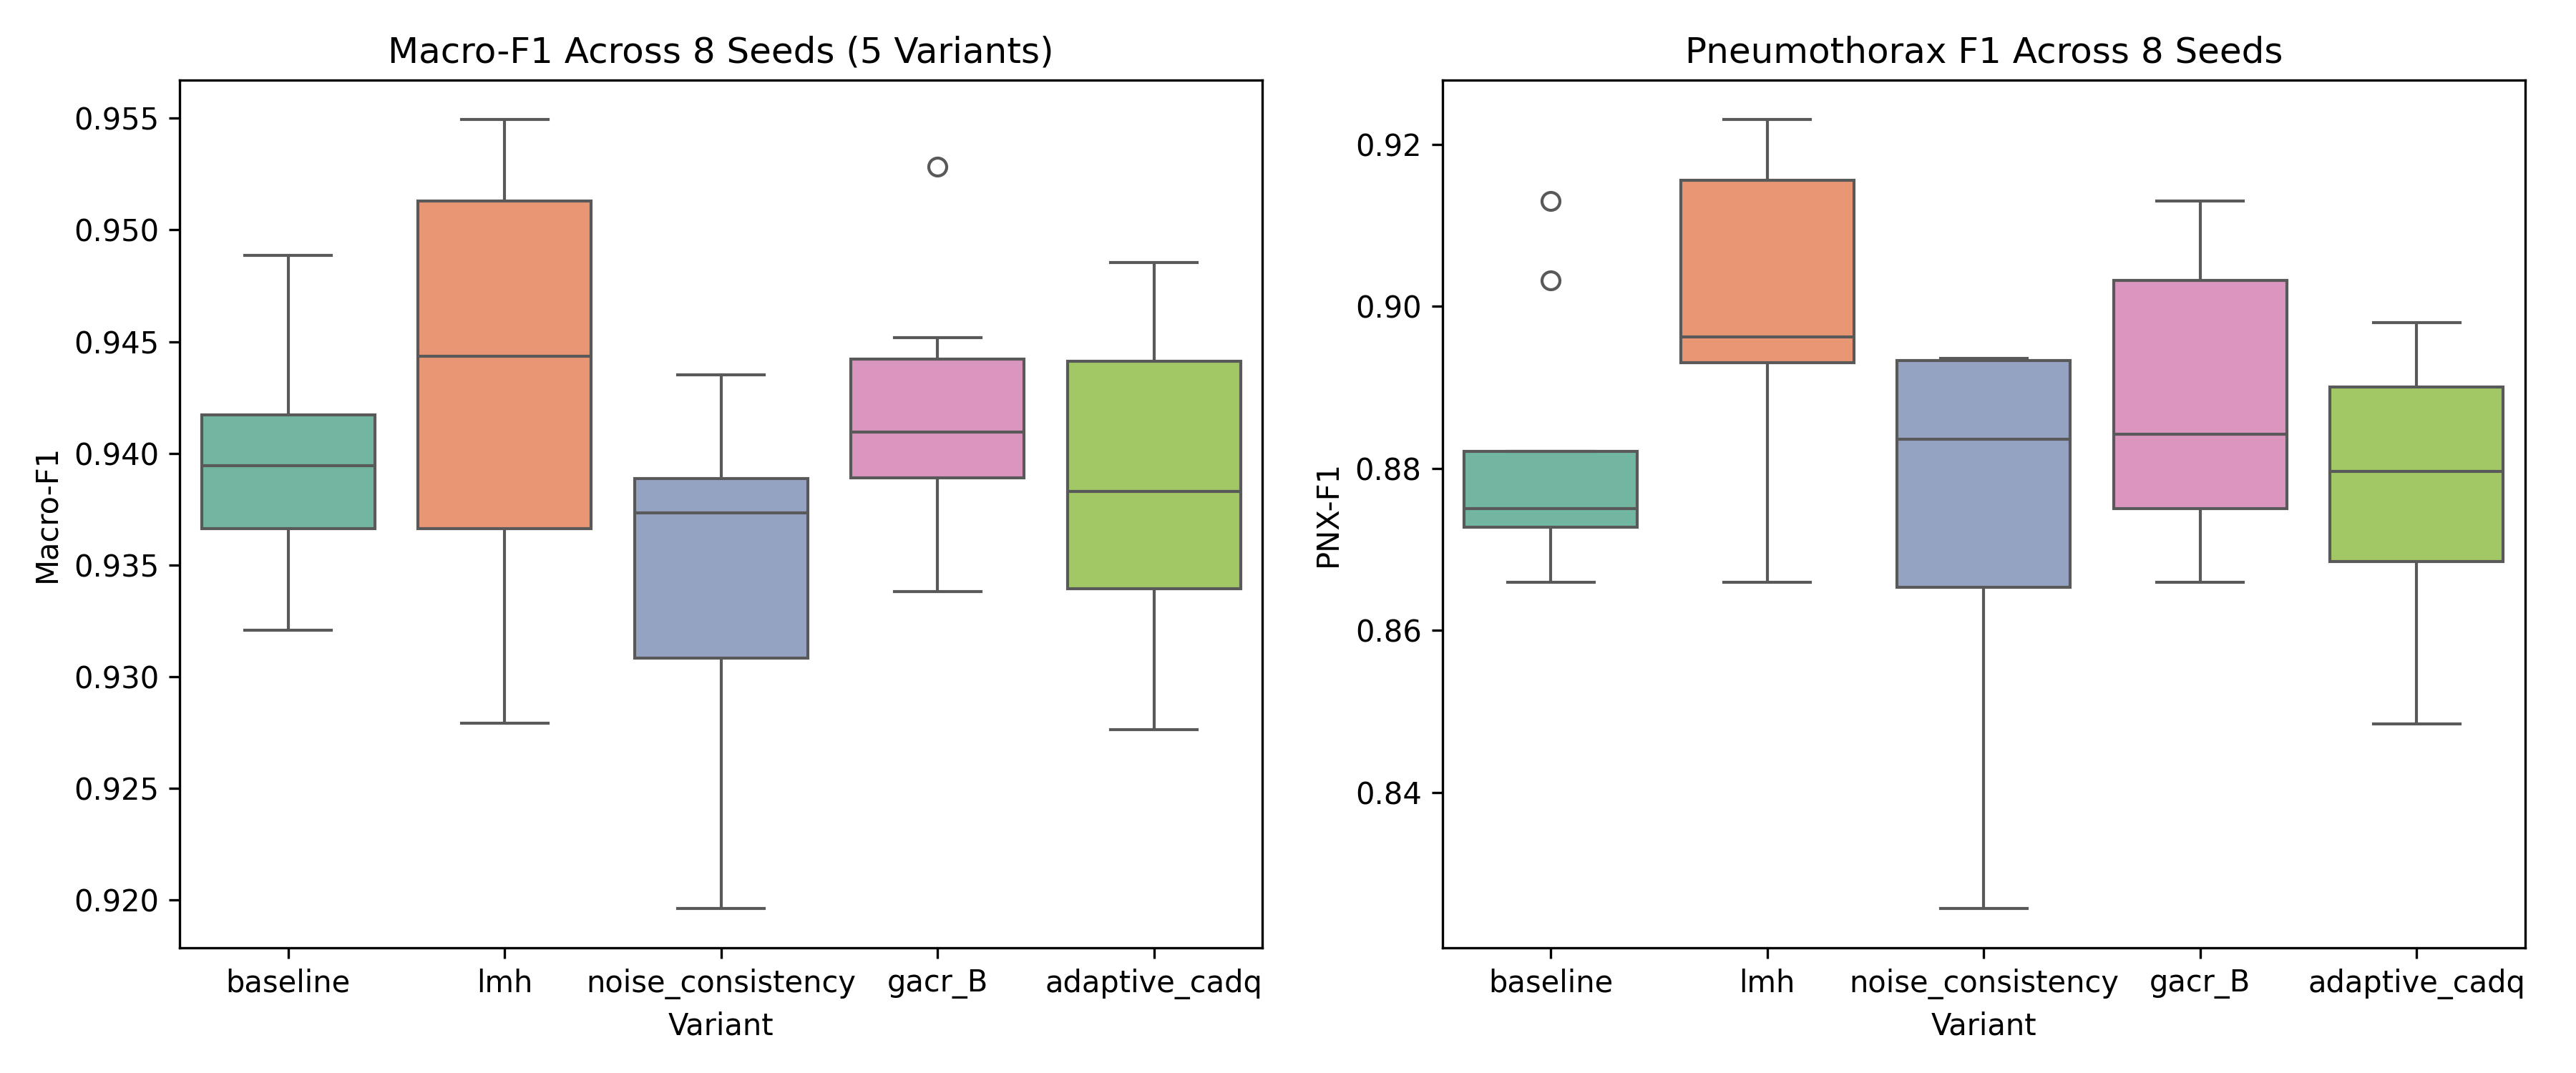
\includegraphics[width=\linewidth]{figures/f1_boxplots.png}
\caption{Macro-F1 and Pneumothorax F1 distributions across eight seeds.}
\label{fig:f1-boxplots}
\end{figure}

No Macro-F1 variant contrast remained significant after Benjamini--Hochberg
correction. The largest unadjusted signal was exploratory GACR-B
($\Delta=+0.0020$, Wilcoxon $p=0.0547$, false-discovery rate (FDR)
$p=0.2188$). LMH reduced AUROC by 0.0126 (FDR $p=0.000012$), and
Noise-Consistency by 0.0014 (FDR $p=0.0044$); Adaptive-CADQ did not differ
from baseline (FDR $p=0.8438$). LMH increased
ECE by 0.0384 and Brier by 0.0163 (FDR $p=0.0313$ and $0.0156$). Noise-
Consistency increased Brier by 0.0133 (FDR $p=0.0156$), while its ECE change
was inconclusive.

\begin{table}[pos=htbp]
\centering
\caption{Paired comparison $p$-values versus Baseline. Wilcoxon tests use
eight seed-level Macro-F1 values; DeLong uses matched Pneumothorax ROC
predictions (seed 42, the retained probability set); McNemar uses paired
classification decisions on the same 455 studies. No predictions were pooled
across seeds. Values in parentheses are Benjamini--Hochberg adjusted within
each test family.}
\label{tab:pairwise-pvalues}
\scriptsize
\resizebox{\linewidth}{!}{%
\begin{tabular}{lccc}
\toprule
Condition & Wilcoxon Macro-F1 $p$ (BH) & DeLong PNX AUROC $p$ (BH) & McNemar $p$ (BH)\\
\midrule
LMH (PoE) & 0.2500 (0.3333) & $<0.0001$ (0.000012) & 0.6936 (1.0000)\\
Noise-Consistency & 0.1953 (0.3333) & 0.0022 (0.0044) & 0.0754 (0.3018)\\
GACR-B (exploratory) & 0.0547 (0.2188) & 0.0315 (0.0420) & 1.0000 (1.0000)\\
Adaptive-CADQ & 0.8438 (0.8438) & 0.7304 (0.7304) & 1.0000 (1.0000)\\
\bottomrule
\end{tabular}}
\end{table}



GACR-B and Adaptive-CADQ produced zero prediction discordance with Baseline
across all 455 held-out studies (McNemar $p=1.000$ for each). Thus, despite
different loss functions and training dynamics, these variants yielded
byte-identical decisions on the test set. This result is consistent with a
text-dominated optimization landscape in which the report shortcut acts as a
single attractor; it is not evidence that the image pathway is intrinsically
non-functional in other cohorts.

Mean row-normalized baseline recalls were 97.78\% (Normal), 95.54\%
(Pneumonia), and 89.36\% (Pneumothorax). LMH improved Normal recall but reduced
Pneumothorax recall; Noise-Consistency showed the reverse trade-off.

\begin{figure}[pos=htbp]
\centering
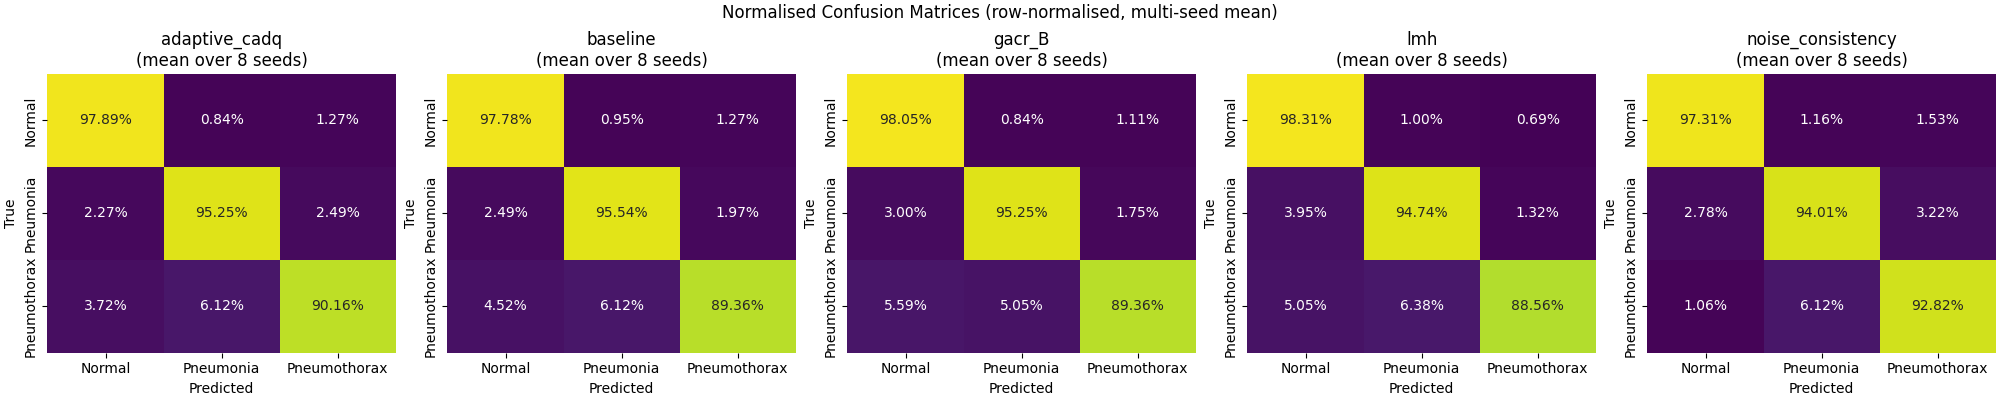
\includegraphics[width=\linewidth]{figures/confusion_matrices_normalised.png}
\caption{Row-normalized confusion matrices aggregated across the eight seeds.
Each matrix is normalized by the true-class row; the displayed aggregate is
descriptive because the same held-out studies recur across seeds.}
\label{fig:confusion-matrices}
\end{figure}

\begin{figure}[pos=htbp]
\centering
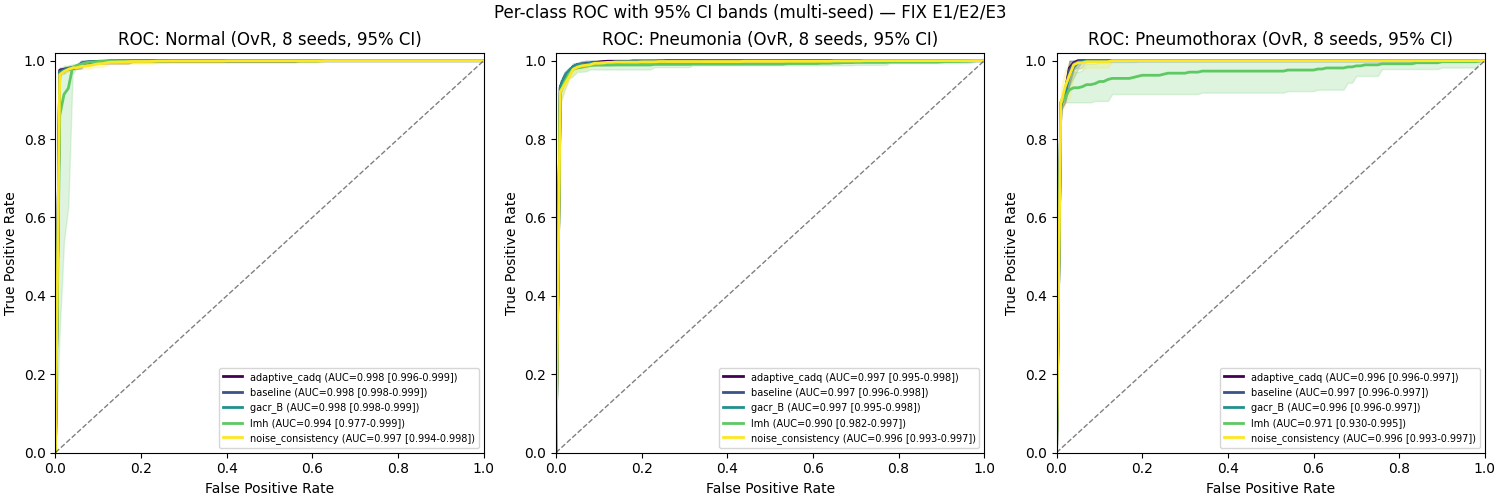
\includegraphics[width=\linewidth]{figures/roc_curves_with_ci.png}
\caption{Per-class ROC curves with descriptive multi-seed 95\% bands. Significant
DeLong $p$-values for LMH and Noise-Consistency reflect AUROC degradation
relative to Baseline, not improvement; all DeLong comparisons use matched
seed-level predictions.}
\label{fig:roc-curves}
\end{figure}

The baseline reliability error was $0.0237\pm0.0048$ and Brier score
$0.0522\pm0.0040$; LMH was less calibrated. Reliability and ROC displays are
descriptive because the same studies recur across seeds.

\begin{figure}[pos=htbp]
\centering
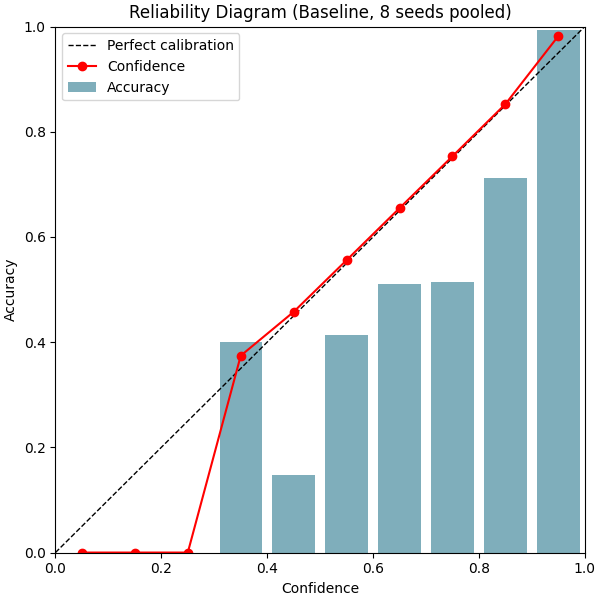
\includegraphics[width=0.50\linewidth]{figures/reliability_diagram.png}
\caption{Descriptive baseline reliability diagram.}
\label{fig:reliability}
\end{figure}

\begin{figure}[pos=htbp]
\centering
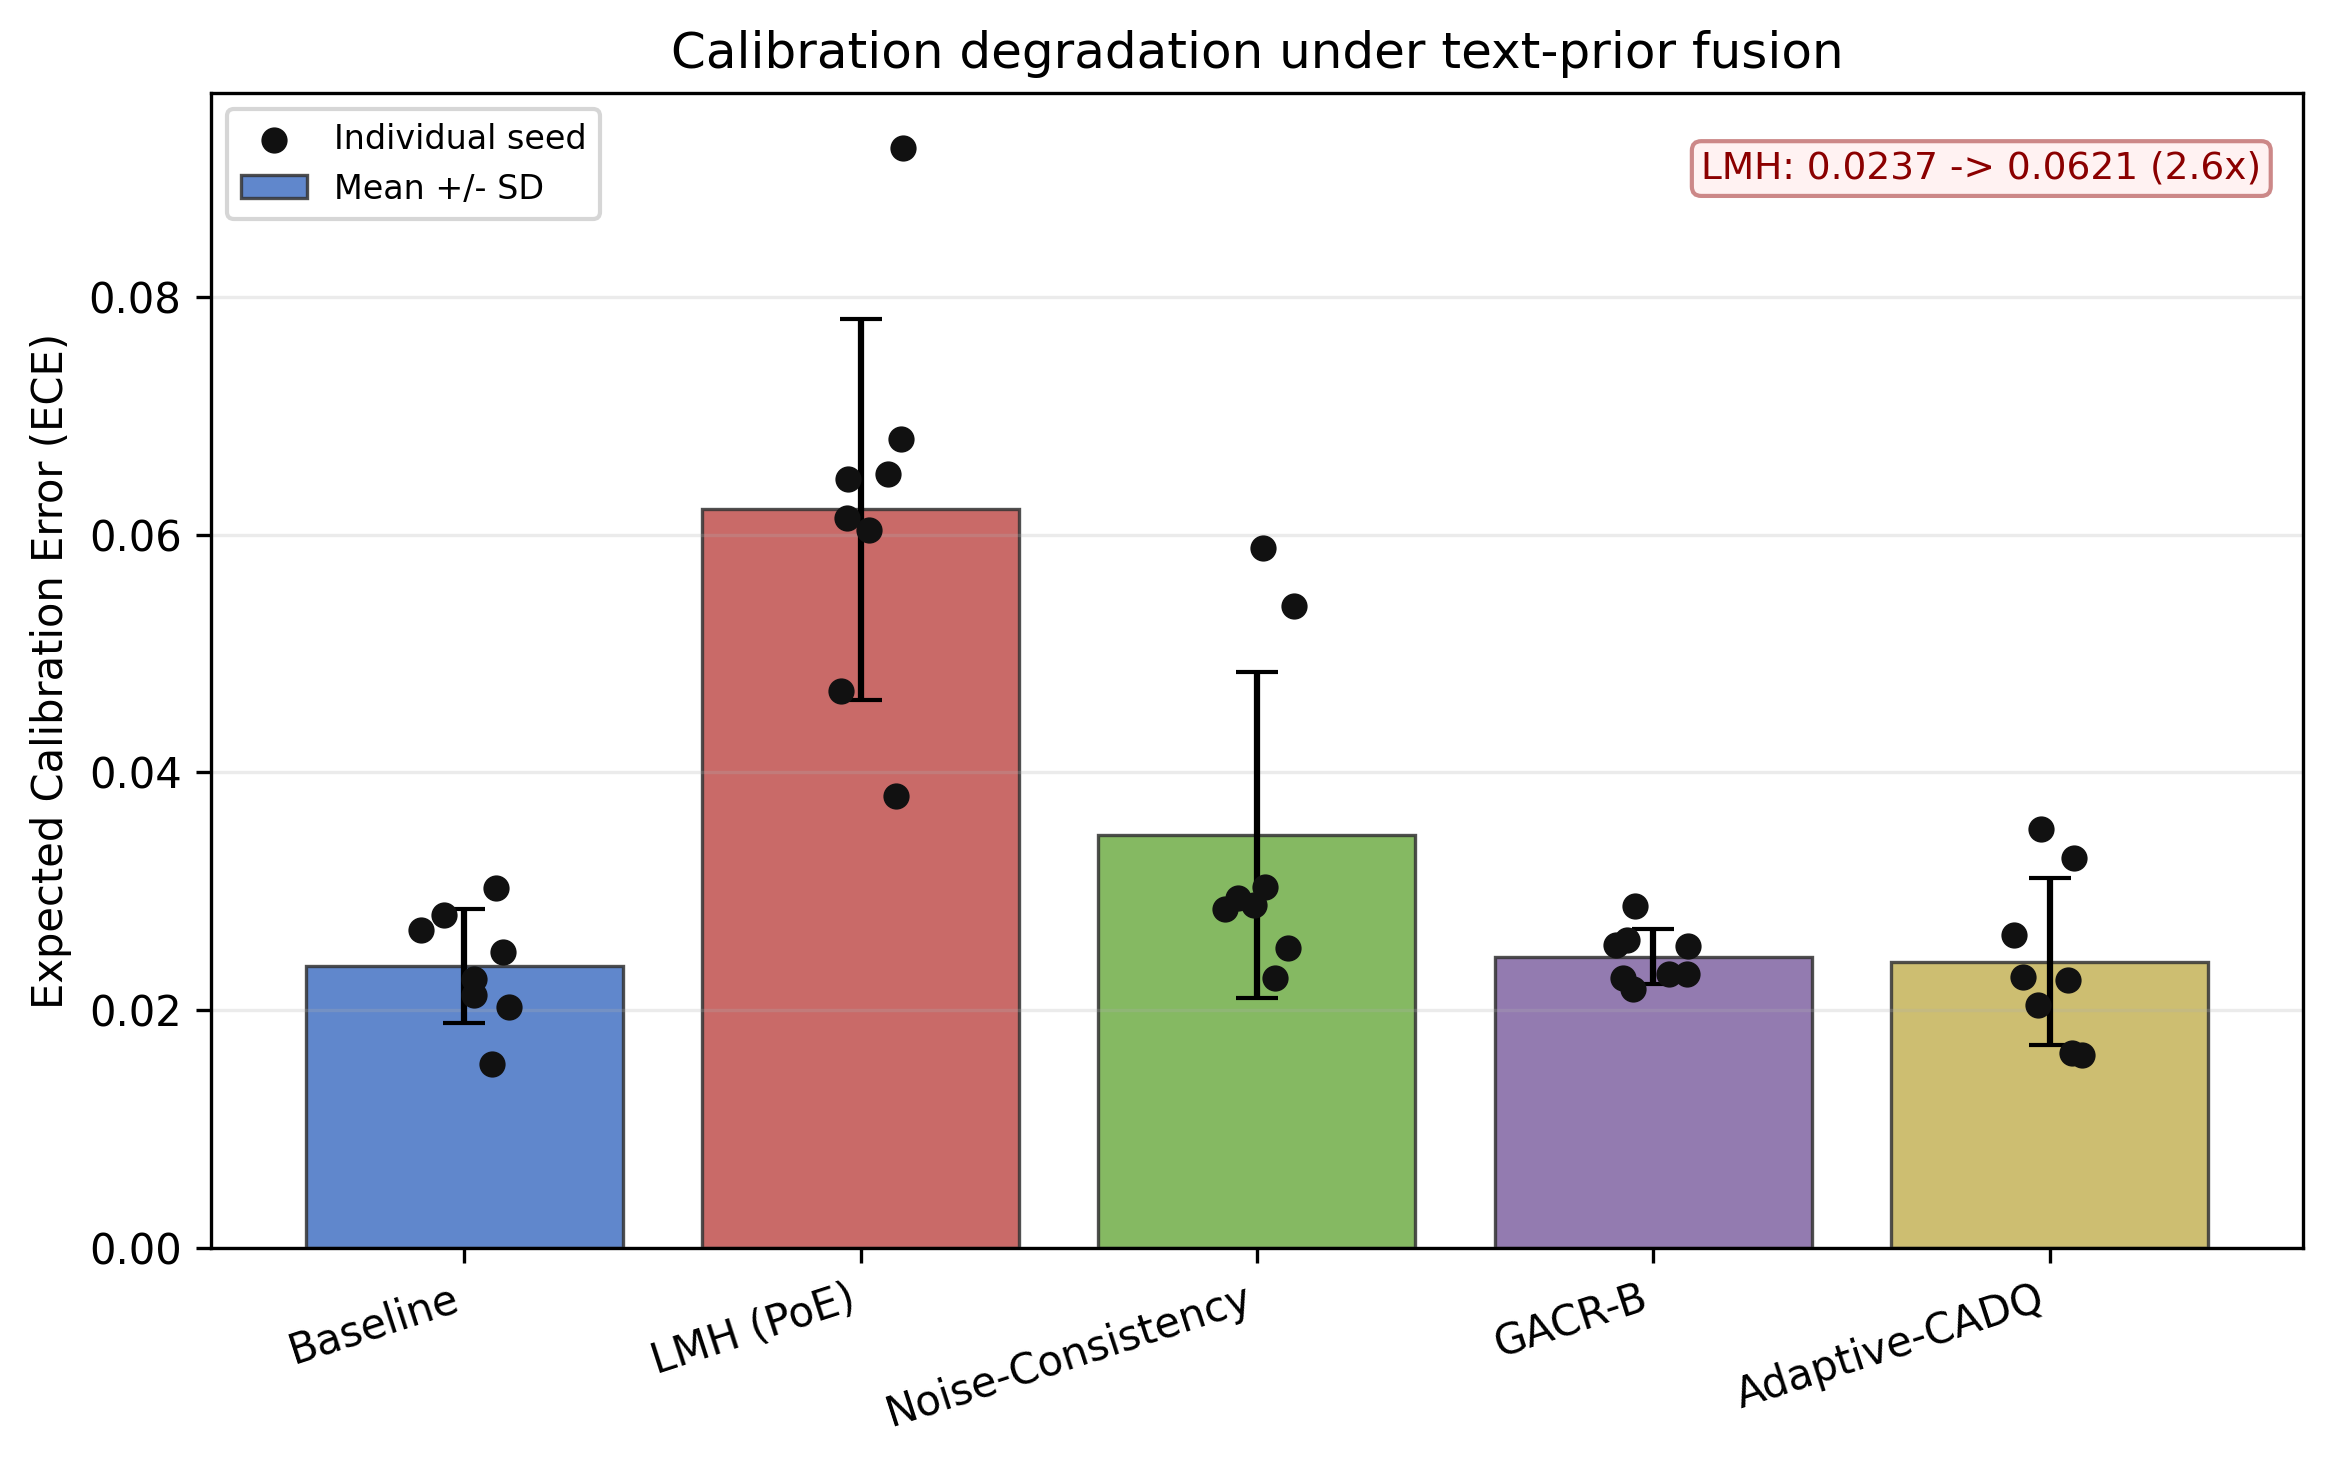
\includegraphics[width=0.68\linewidth]{figures/ece_seed_dots.png}
\caption{Expected calibration error (ECE) by condition with individual seed
values. LMH increases ECE from 0.0237 to 0.0621 (2.6-fold); bars show mean
$\pm$ SD across eight seeds.}
\label{fig:ece-seed-dots}
\end{figure}

\subsection{Controls and report-preserving ablation}\label{sec:results-controls}
The retained image-only control achieved Macro-F1 0.4611, accuracy 0.5670, and
AUROC 0.6728; text-only achieved 0.8555 and 0.9820, respectively. Gray-Square
retained Macro-F1 0.9381, accuracy 0.9604, and AUROC 0.9960, only 0.0015 below
the baseline mean. These are single saved runs, and image-only checkpoint
selection was imperfect, so the controls are diagnostic rather than modality
rankings.

\begin{table}[pos=htbp]
\centering
\caption{Retained control outputs on the 455-study test set (single runs).}
\label{tab:controls}
\small
\begin{tabular}{lccccc}
\toprule
Control & Macro-F1 & Accuracy & Macro-AUROC & ECE & Brier\\
\midrule
Image-only & 0.4611 & 0.5670 & 0.6728 & 0.0993 & 0.6142\\
Text-only & 0.8555 & 0.9077 & 0.9820 & 0.0203 & 0.1289\\
Gray-Square & 0.9381 & 0.9604 & 0.9960 & 0.0369 & 0.0589\\
\bottomrule
\end{tabular}
\end{table}

\begin{figure}[pos=htbp]
\centering
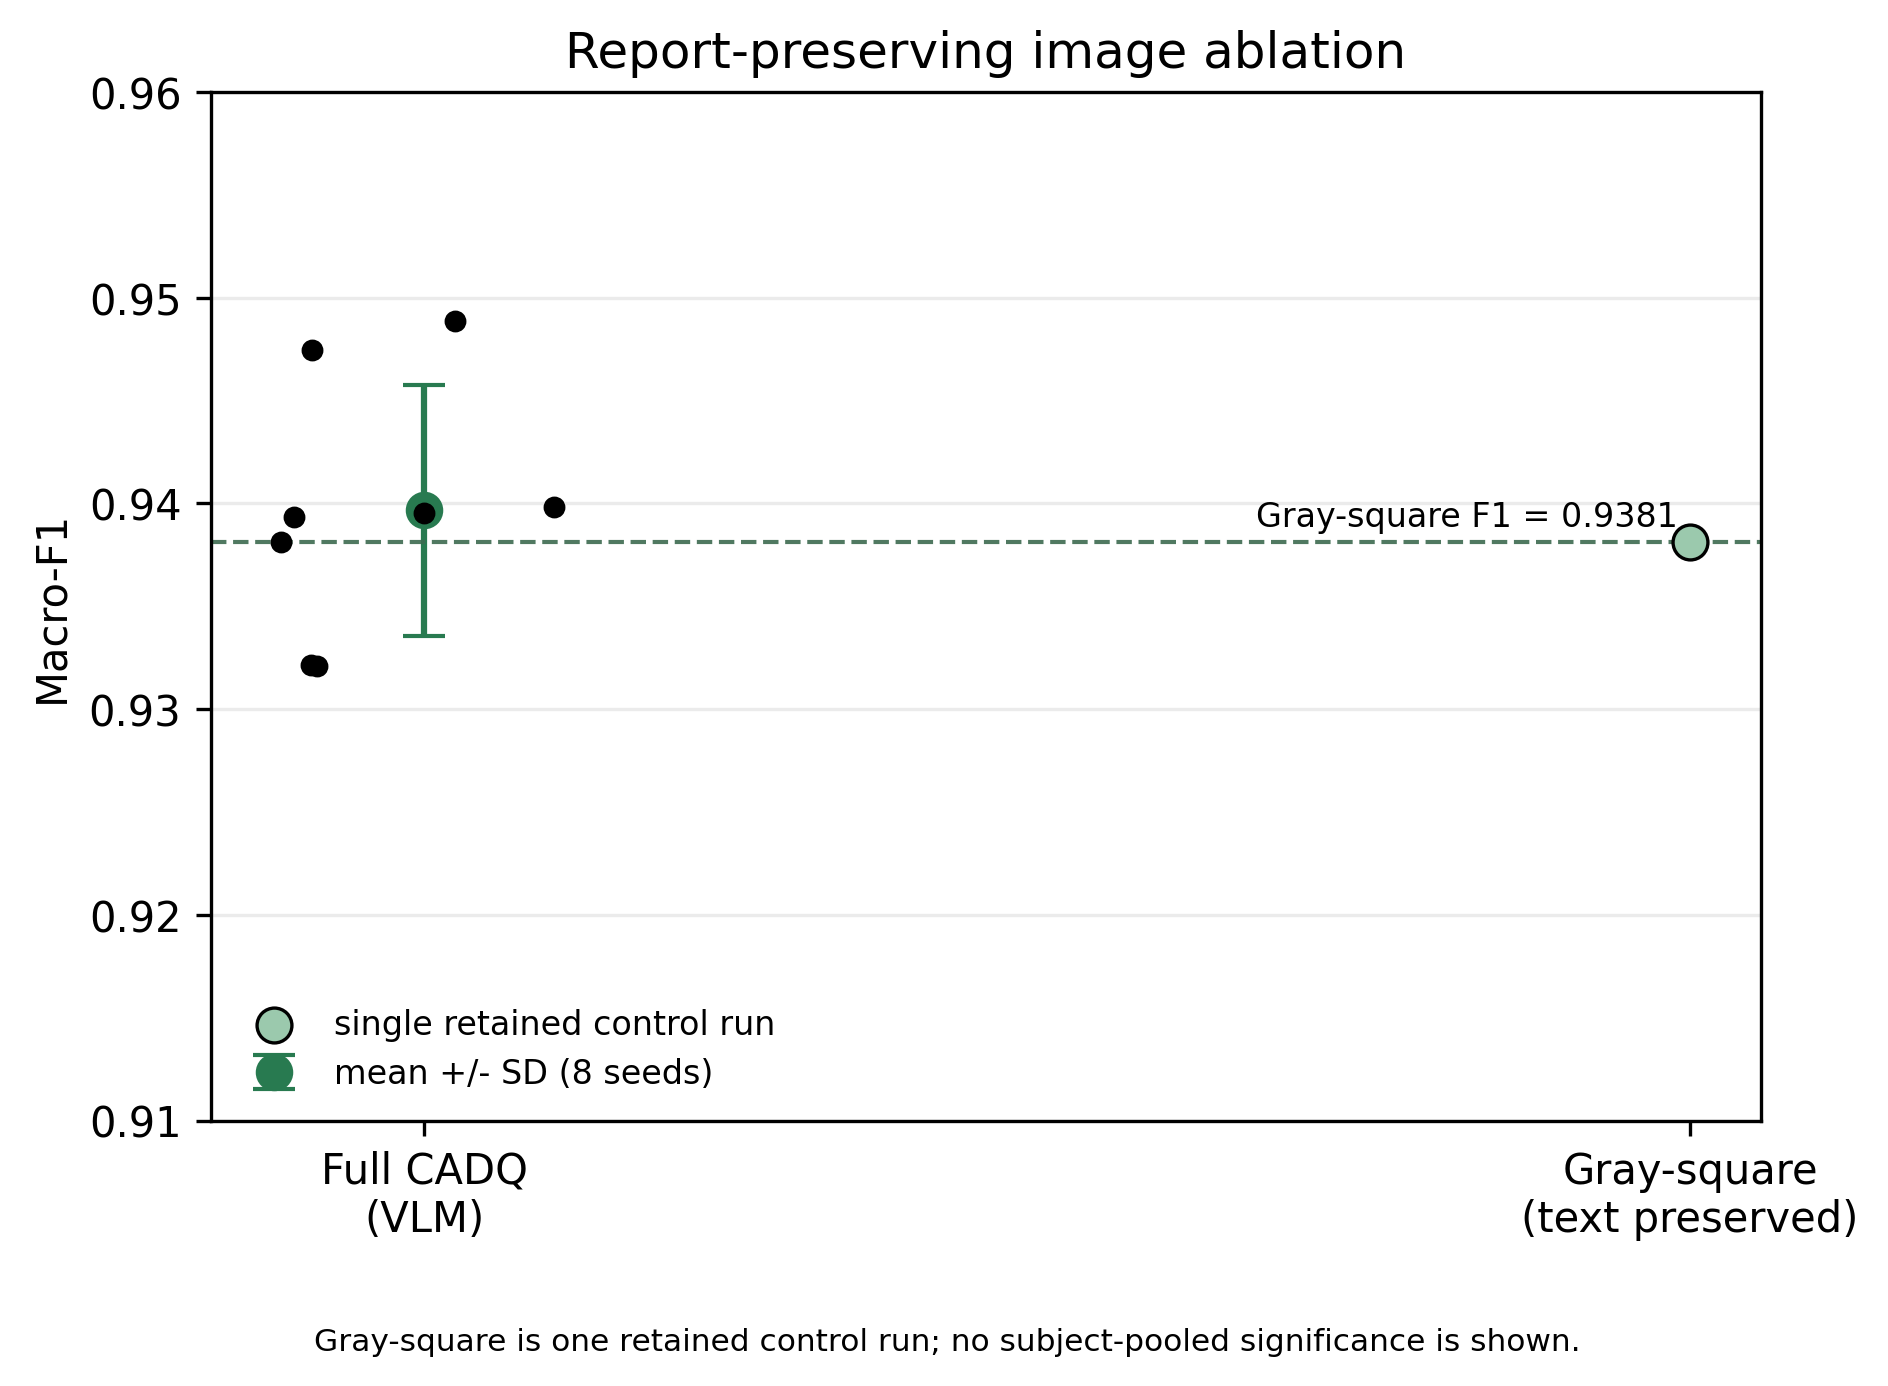
\includegraphics[width=0.66\linewidth]{figures/circularity_contrast.png}
\caption{Report-preserving image ablation; Gray-Square is one retained run.}
\label{fig:circularity-contrast}
\end{figure}

\begin{figure}[pos=htbp]
\centering
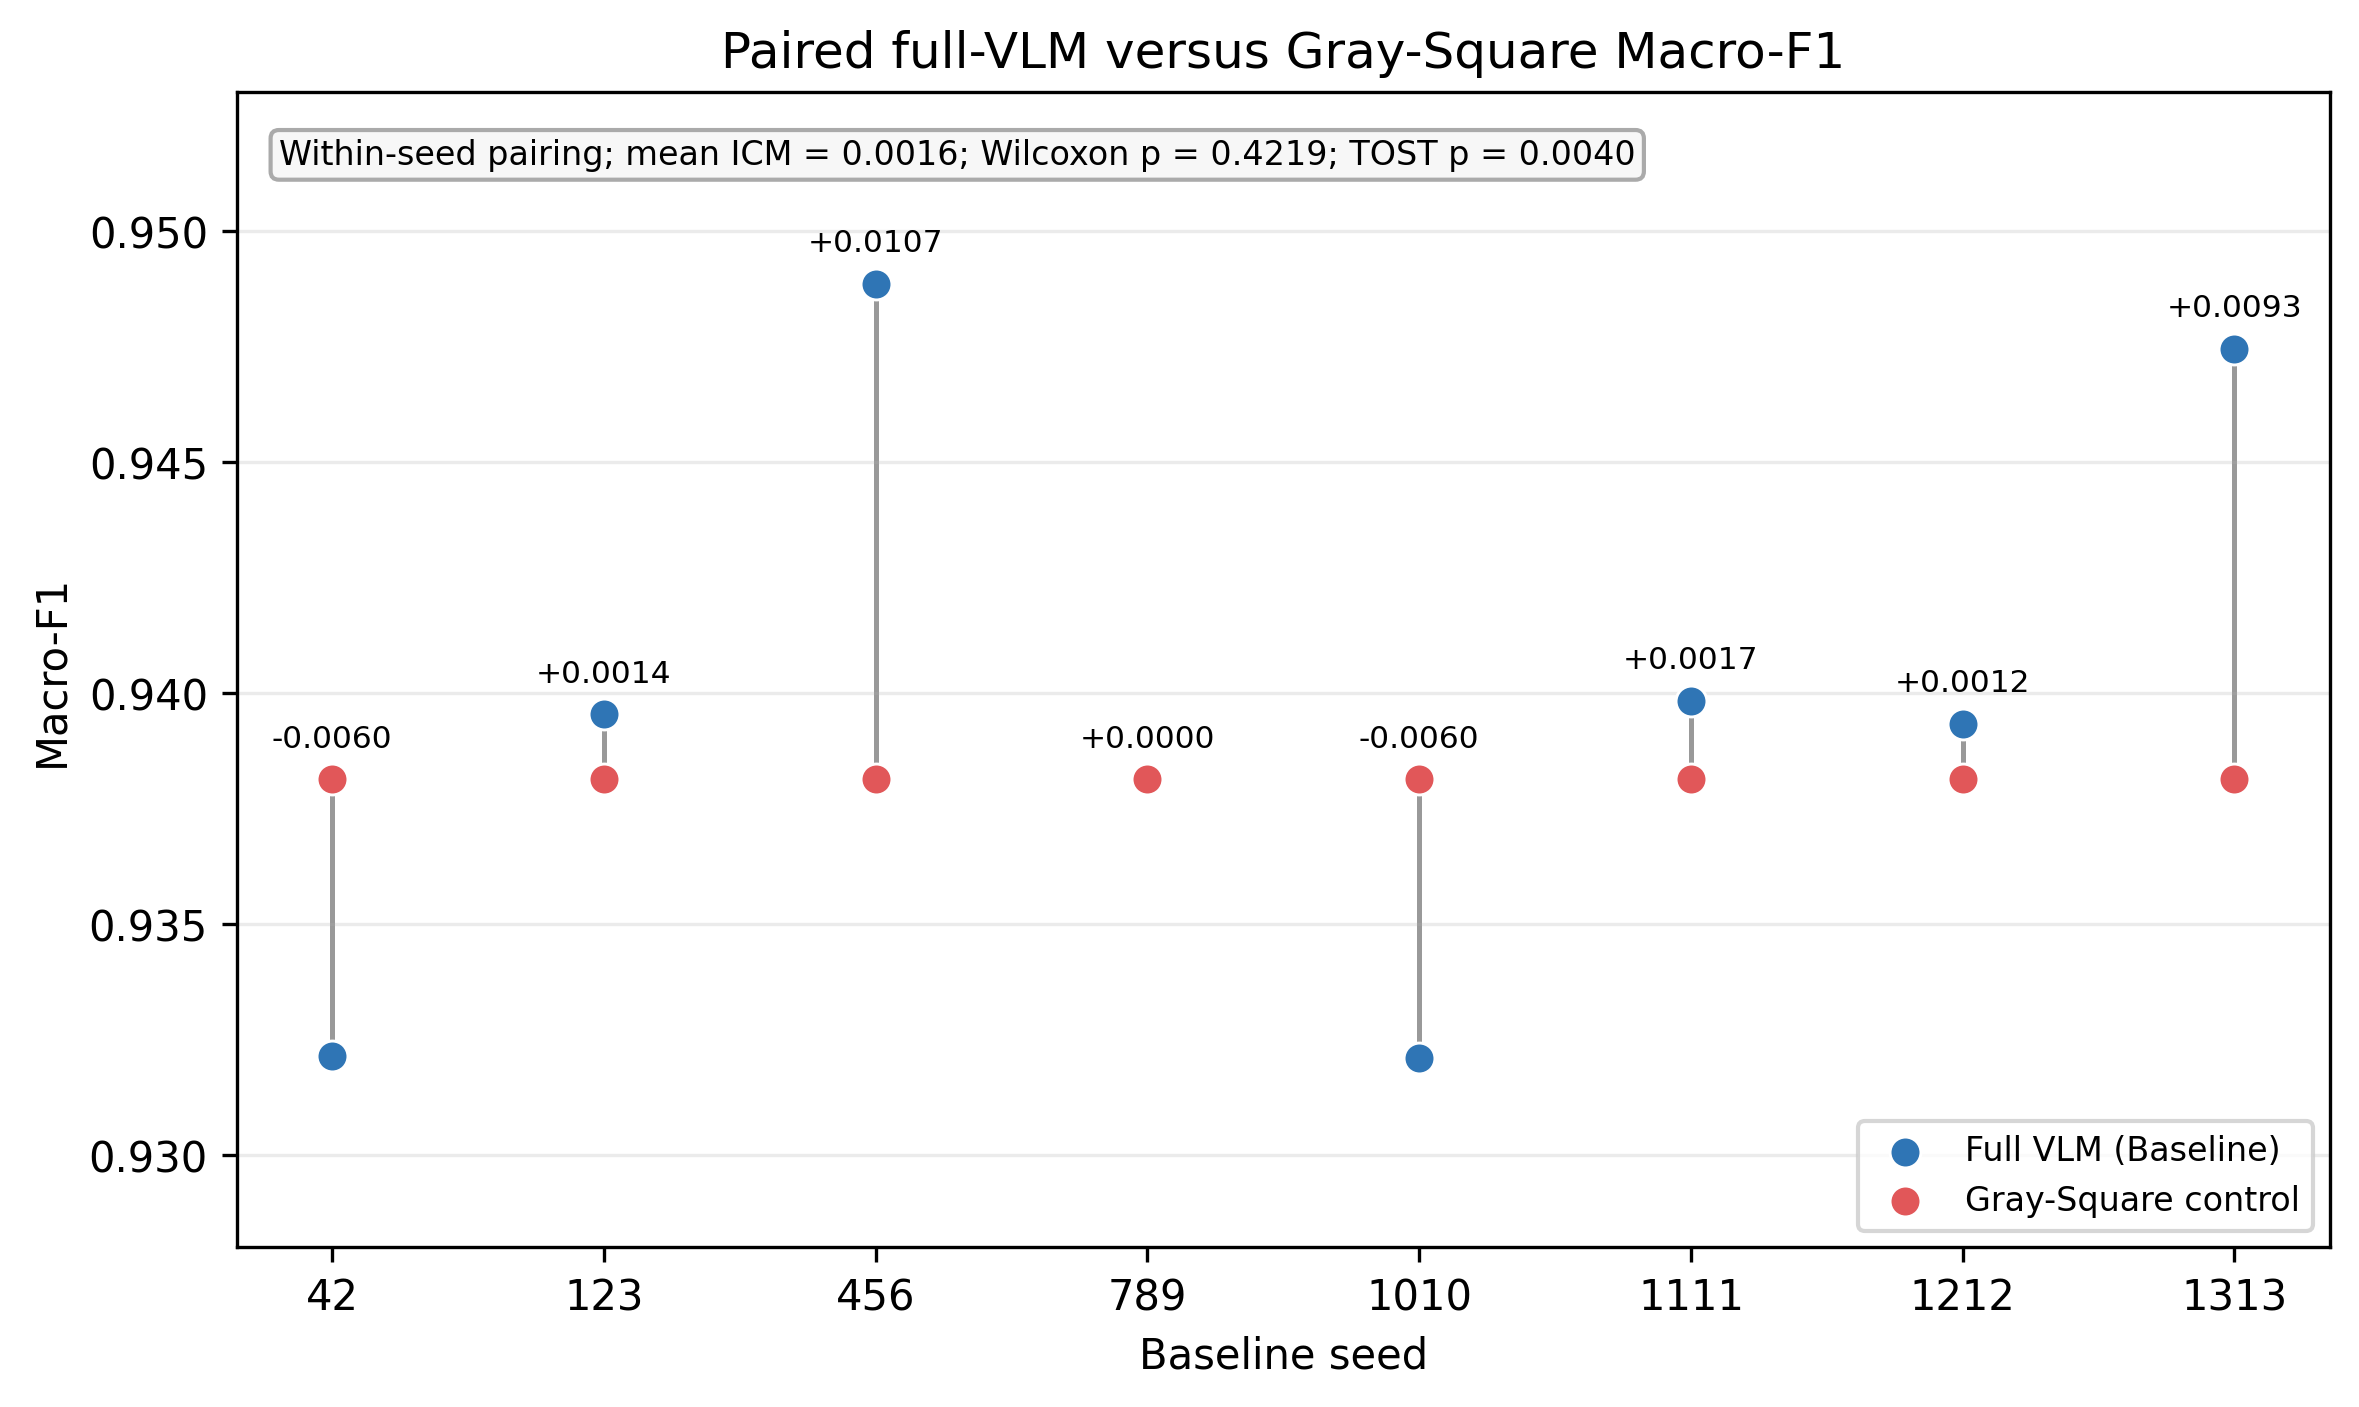
\includegraphics[width=0.70\linewidth]{figures/paired_vlm_gray_square.png}
\caption{Paired Baseline VLM and Gray-Square Macro-F1 for the eight baseline
seeds. Lines connect the two predictions for the same seed; the small paired
differences make the near-zero ICM visible.}
\label{fig:paired-vlm-gray}
\end{figure}

\subsection{Image Contribution Metric}\label{sec:results-icm}
With Gray-Square as reference, baseline ICM was $0.0016\pm0.0065$ (median
0.0014). The bootstrap 95\% confidence interval (CI) was
$[-0.0026,0.0061]$. The signed Wilcoxon test did not
reject zero ($p=0.4219$), while TOST supported equivalence within
$[-0.01,0.01]$ ($p=0.0040$, Cohen’s $d=0.247$). LMH had ICM
$0.0056\pm0.0098$ (TOST $p=0.1223$); Noise-Consistency $-0.0039\pm0.0081$
(TOST $p=0.0345$); Adaptive-CADQ $0.0007\pm0.0077$ (TOST $p=0.0054$); and
exploratory GACR-B $0.0038\pm0.0062$ (TOST $p=0.0122$). None demonstrated a
robust increase in incremental image contribution.

\begin{table}[pos=htbp]
\centering
\caption{Image Contribution Metric (ICM) statistics by condition (eight seeds).
Confidence intervals are percentile bootstrap intervals from 2,000 resamples;
Wilcoxon tests are signed-rank tests against zero; TOST tests equivalence to
zero within $[-0.01,0.01]$.}
\label{tab:icm-statistics}
\scriptsize
\resizebox{\linewidth}{!}{%
\begin{tabular}{lrrrrrrr}
\toprule
Condition & Mean & SD & Median & 95\% CI & Wilcoxon $p$ & TOST $p$ & Cohen's $d$\\
\midrule
Baseline & 0.0016 & 0.0065 & 0.0014 & [-0.0026, 0.0061] & 0.4219 & 0.0040 & 0.247\\
LMH (PoE) & 0.0056 & 0.0098 & 0.0066 & [-0.0011, 0.0118] & 0.1953 & 0.1223 & 0.566\\
Noise-Consistency & -0.0039 & 0.0081 & -0.0009 & [-0.0097, 0.0009] & 0.3828 & 0.0345 & -0.476\\
GACR-B (exploratory) & 0.0038 & 0.0062 & 0.0030 & [-0.0002, 0.0081] & 0.1953 & 0.0122 & 0.607\\
Adaptive-CADQ & 0.0007 & 0.0077 & 0.0002 & [-0.0043, 0.0057] & 0.8438 & 0.0054 & 0.089\\
\bottomrule
\end{tabular}}
\end{table}

\begin{figure}[pos=htbp]
\centering
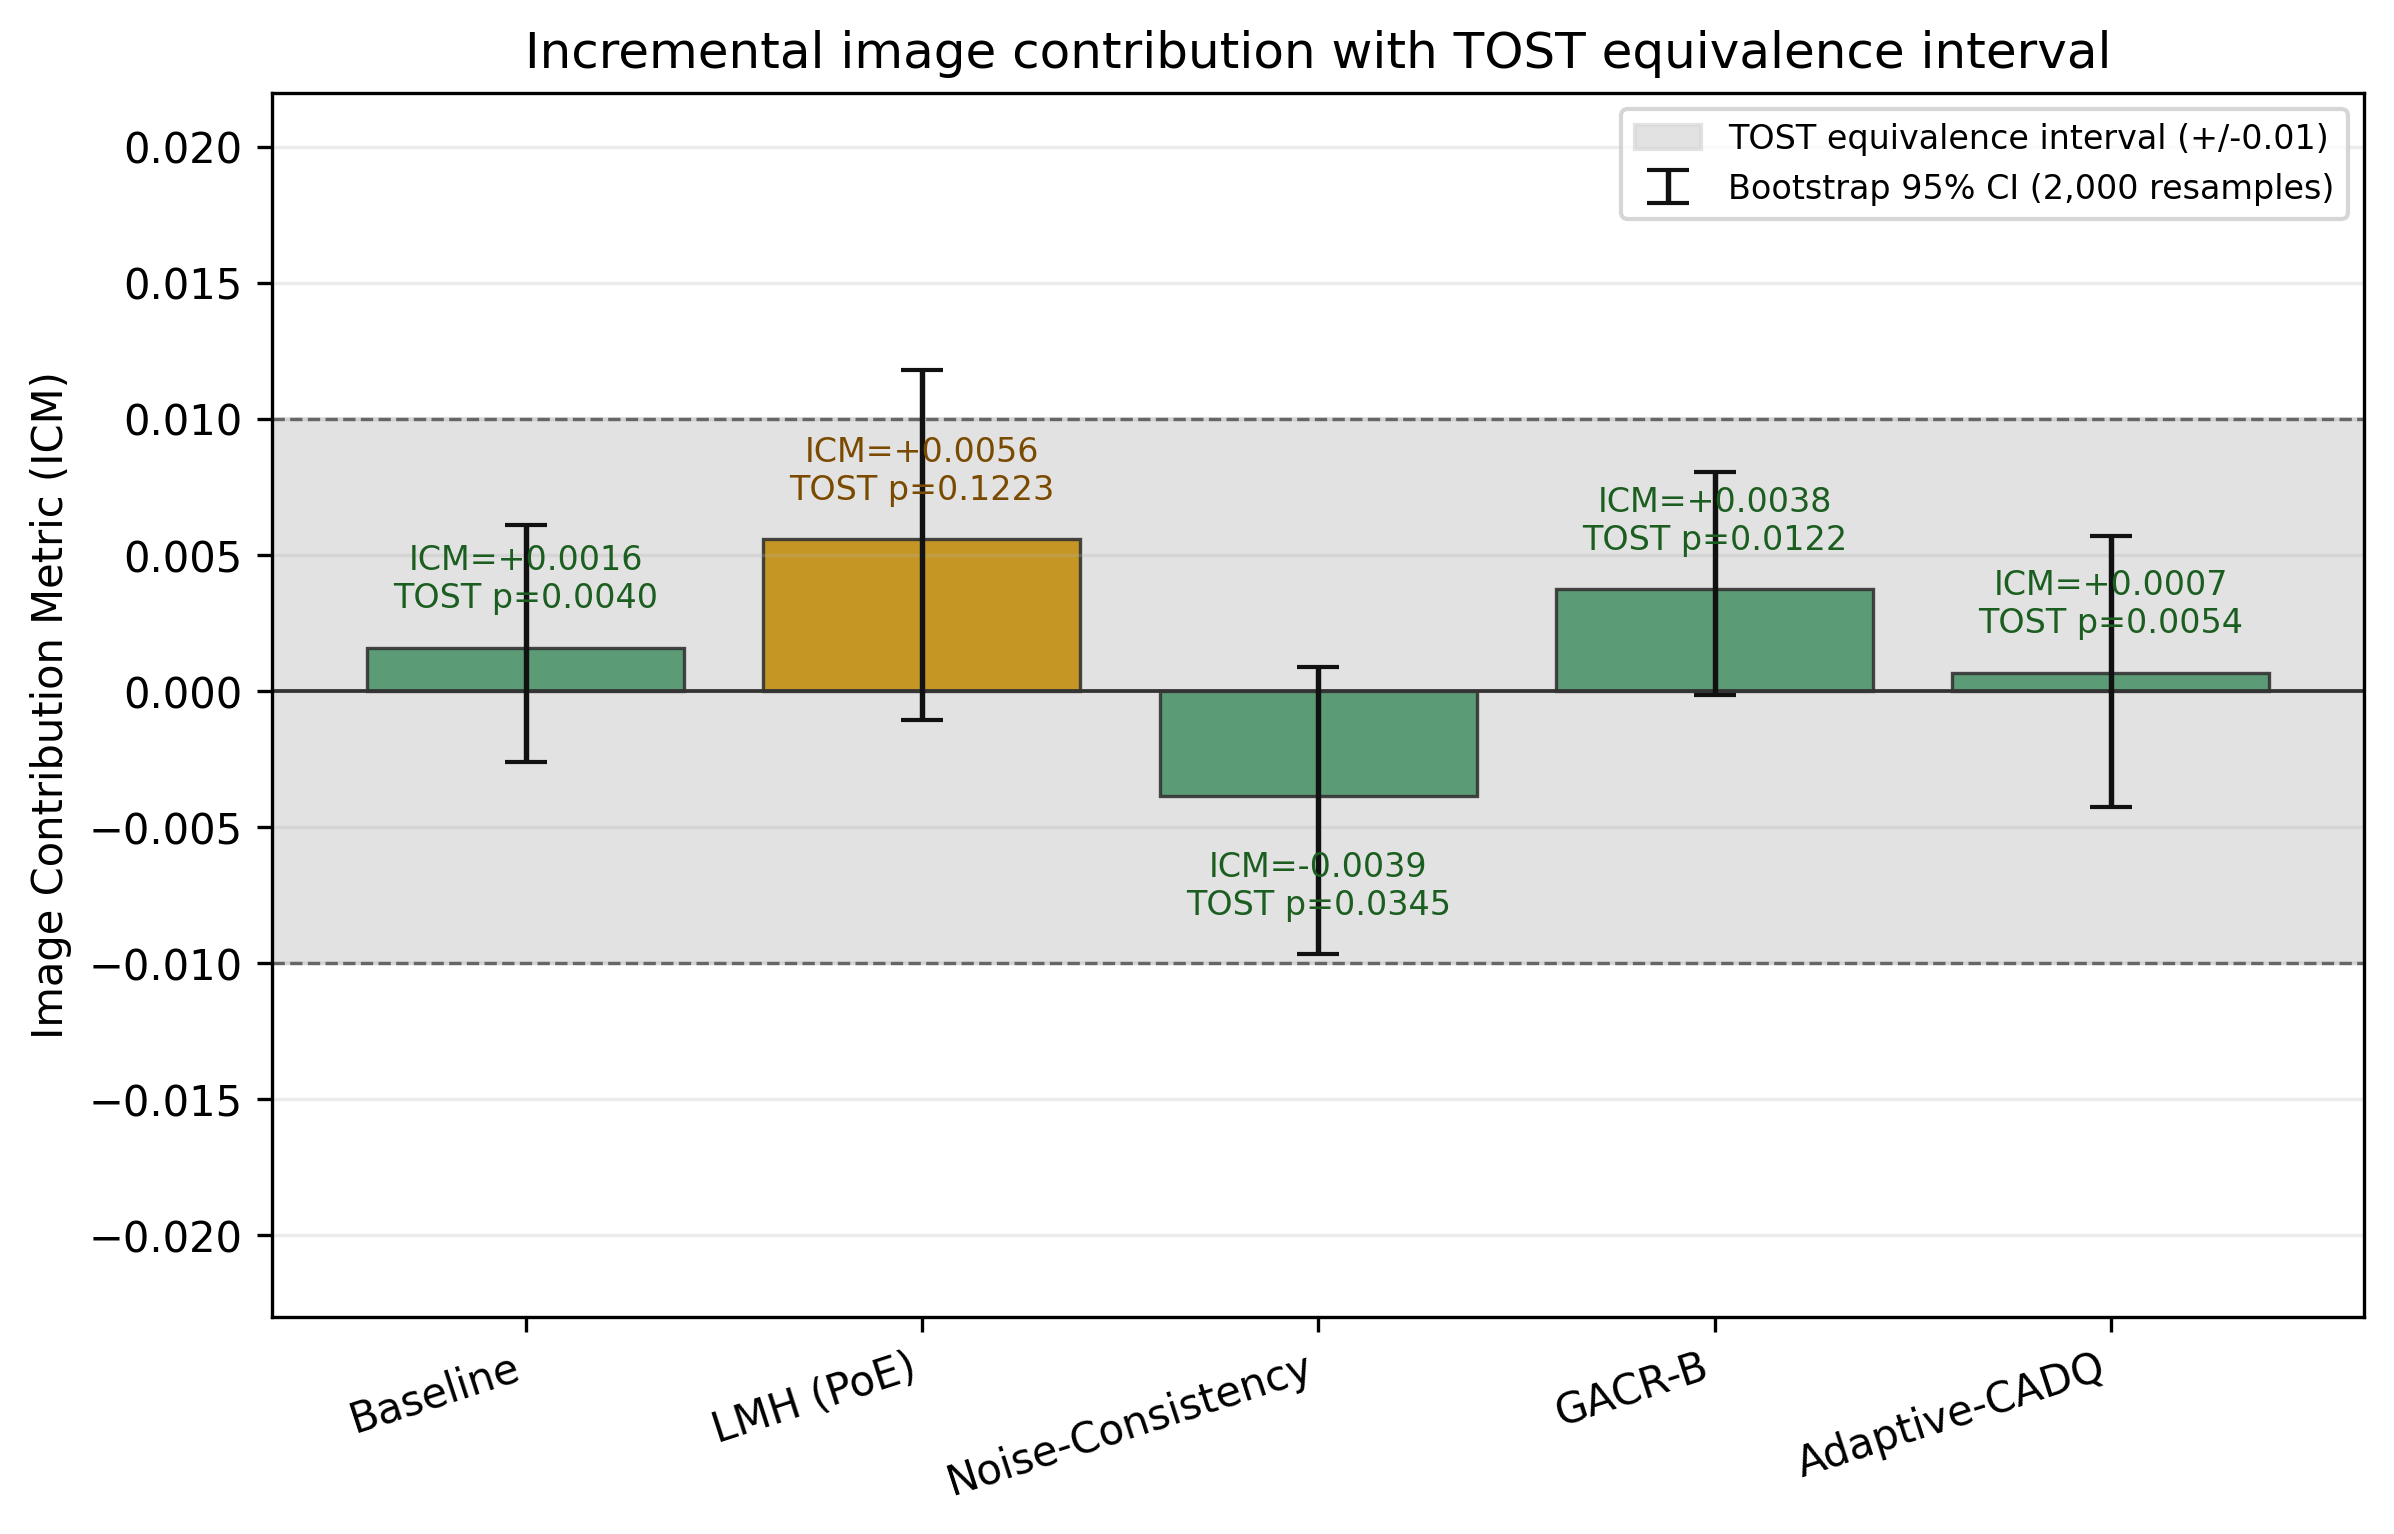
\includegraphics[width=0.70\linewidth]{figures/icm_tost_master.png}
\caption{ICM by condition with percentile bootstrap 95\% confidence intervals.
The shaded band is the pre-specified TOST equivalence interval
$[-0.01,0.01]$; corrected Master statistics are annotated for each condition.}
\label{fig:icm-tost}
\end{figure}

\begin{figure}[pos=htbp]
\centering
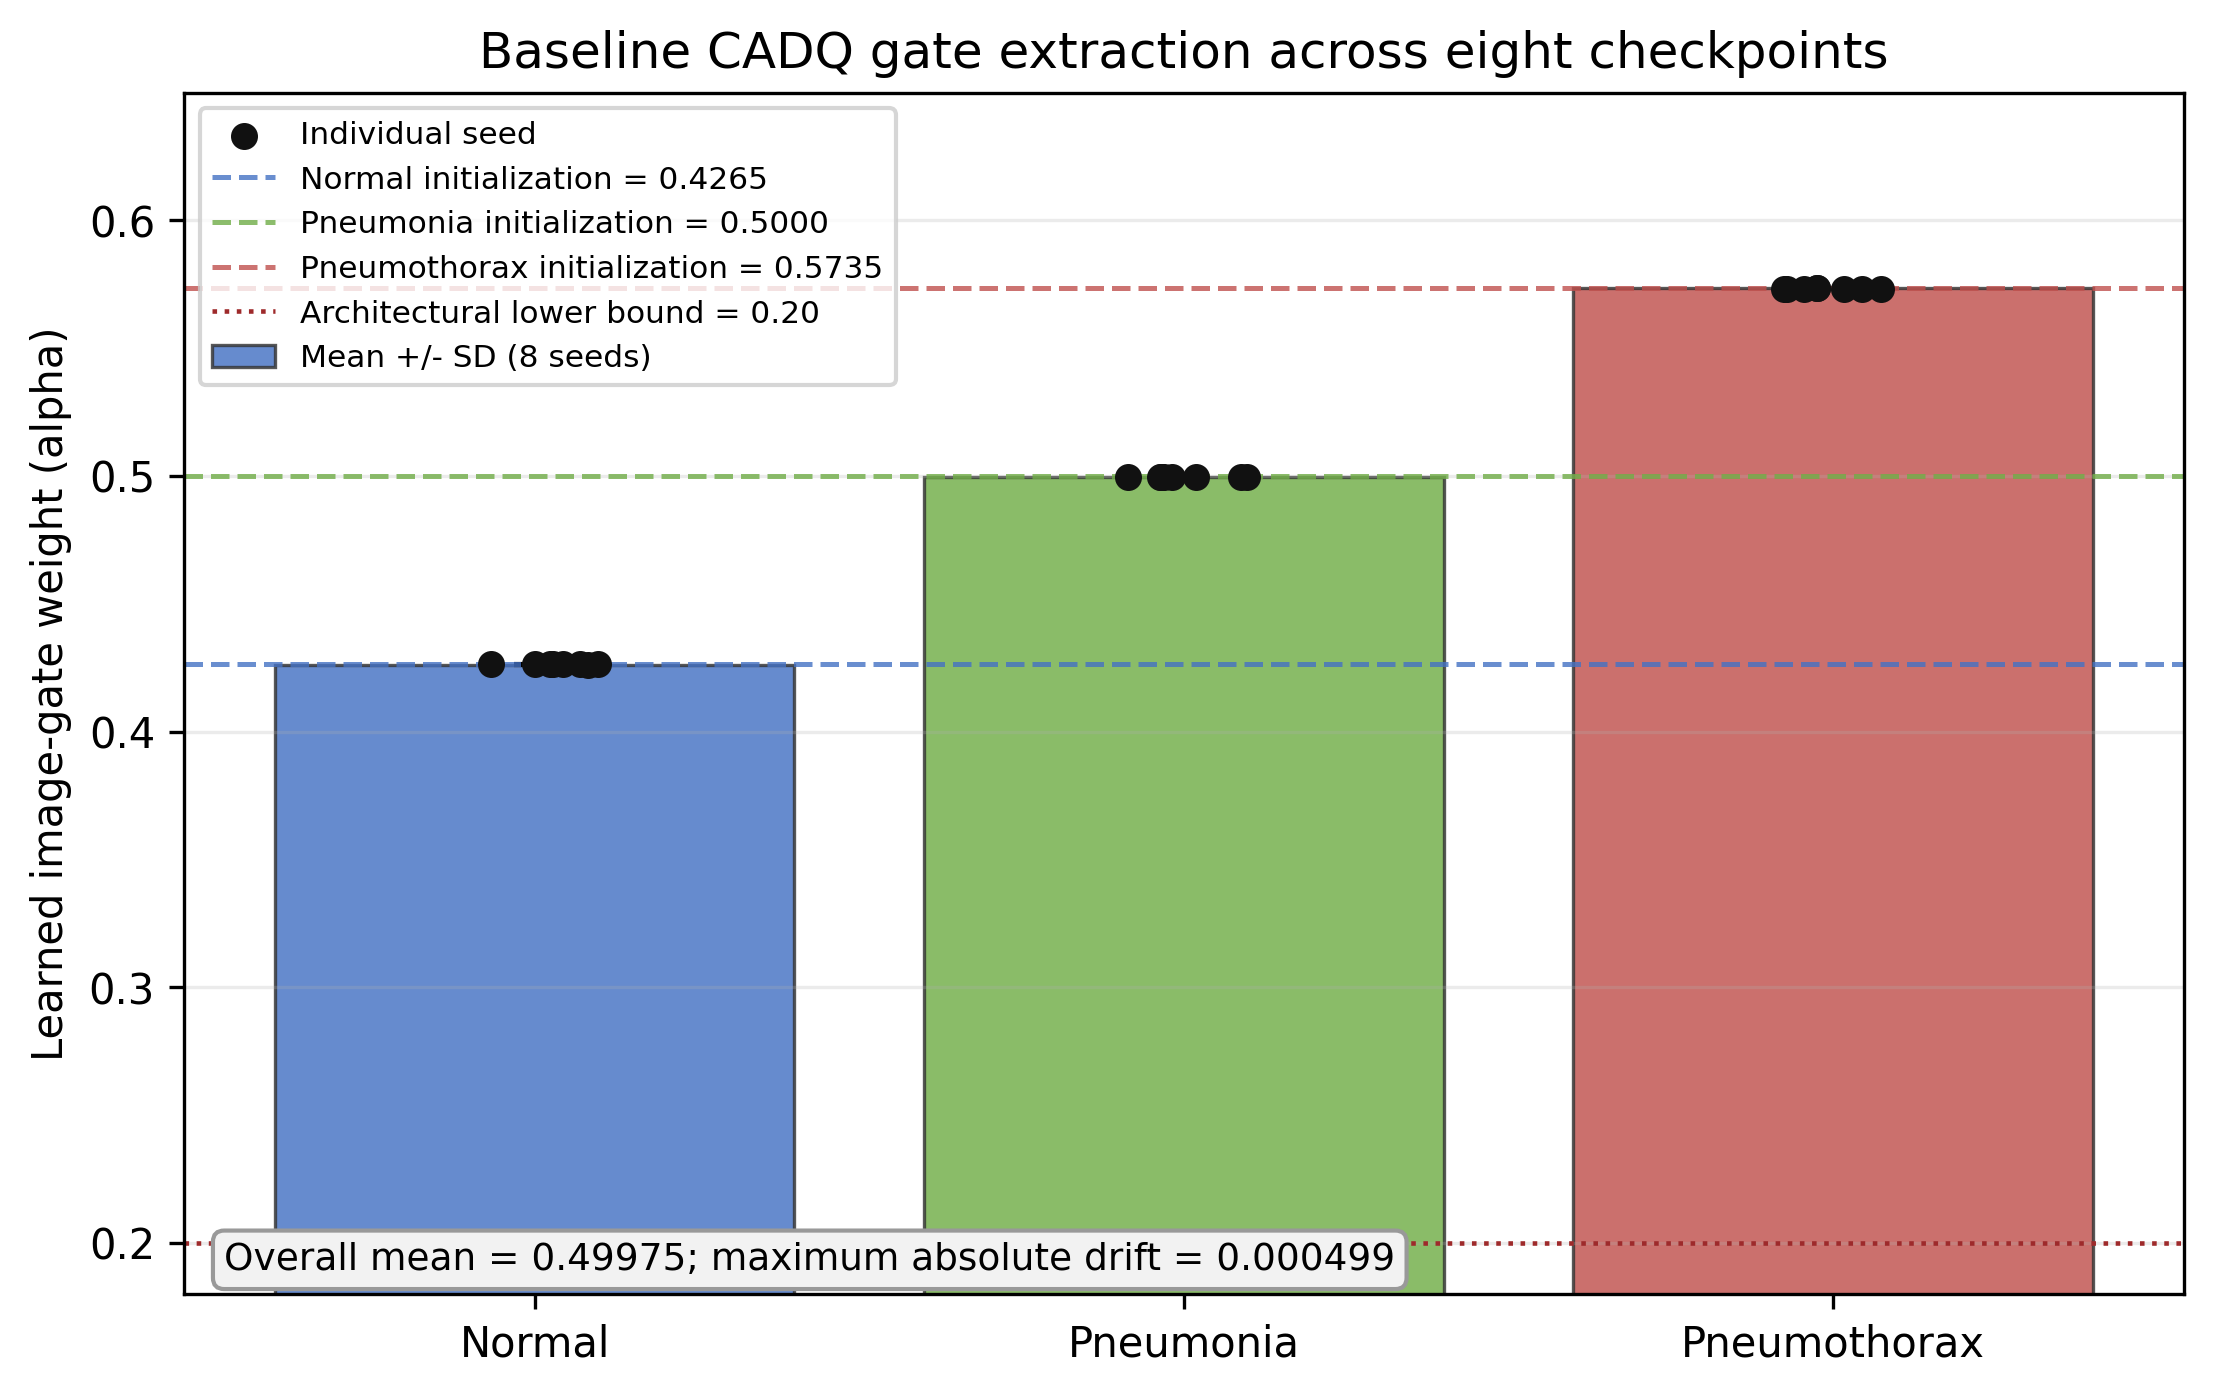
\includegraphics[width=0.70\linewidth]{figures/gate_stagnation_with_dots.png}
\caption{Baseline CADQ image-gate weights extracted from eight checkpoints.
Bars show mean $\pm$ SD, dots show individual seeds, and dashed lines show the
class-specific initialization values computed from the saved checkpoint logits.}
\label{fig:gate-stagnation}
\end{figure}

\subsection{Fusion gates and qualitative inspection}\label{sec:results-gate}
Extracted baseline image-gate means were 0.42624 (Normal), 0.49963
(Pneumonia), and 0.57336 (Pneumothorax), with overall mean 0.49975 versus
0.50000 at initialization. The largest class-wise drift was below 0.0004; the
gate neither collapsed to 0.20 nor demonstrated learned image reliance. Three
Pneumonia Grad-CAM examples (Fig.~\ref{fig:gradcam}) are qualitative only and
do not support localization or causal-grounding claims.

\begin{table}[pos=htbp]
\centering
\caption{Per-seed CADQ gate extraction. Initialization values are computed from
$u=(-0.5,0,0.5)$ and the bounded gate equation; maximum drift is the largest
absolute class-wise deviation from initialization for that seed.}
\label{tab:gate-extraction}
\scriptsize
\setlength{\tabcolsep}{4pt}
\begin{tabular}{r rrr r}
\toprule
Seed & Normal $\alpha$ & Pneumonia $\alpha$ & Pneumothorax $\alpha$ & Max drift\\
\midrule
42   & 0.426270 & 0.499512 & 0.573242 & 0.000488\\
123  & 0.426270 & 0.499512 & 0.573730 & 0.000488\\
456  & 0.426025 & 0.499756 & 0.573242 & 0.000499\\
789  & 0.426270 & 0.499756 & 0.573242 & 0.000255\\
1010 & 0.426270 & 0.499756 & 0.573242 & 0.000255\\
1111 & 0.426270 & 0.499512 & 0.573242 & 0.000488\\
1212 & 0.426270 & 0.499756 & 0.573730 & 0.000255\\
1313 & 0.426270 & 0.499512 & 0.573242 & 0.000488\\
\bottomrule
\end{tabular}
\end{table}

\begin{figure}[pos=htbp]
\centering

\includegraphics[width=0.74\linewidth]{figures/gradcam_baseline.png}
\caption{Qualitative Grad-CAM examples (method of Selvaraju et al. \citep{selvaraju2017gradcam}); no quantitative localization claim.}
\label{fig:gradcam}
\end{figure}

Overall, high performance persisted after image replacement, baseline ICM was
near zero, and the gate remained near initialization. This pattern is
consistent with report-linked shortcut potential in this cohort, not a
universal claim that multimodal models ignore images.

% MedVision manuscript -- Discussion section

\section{Discussion}\label{sec:discussion}

\subsection{Principal findings}\label{sec:discussion-principal}
The central result was a mismatch between high predictive performance and
incremental image evidence. Gray-Square retained Macro-F1 0.9381 versus the
baseline eight-seed mean of $0.9397\pm0.0061$; baseline ICM was
$0.0016\pm0.0065$, with a non-significant signed test and TOST equivalence to
the operational interval $[-0.01,0.01]$. Thus, replacing the radiograph changed
little under this intervention. It does not imply that radiographs are
universally unused.

The tested interventions did not provide a consistent remedy. LMH had the
highest Macro-F1 but lower AUROC and substantially worse ECE and Brier score;
Noise-Consistency also increased Brier score without increasing ICM.
Adaptive-CADQ remained near baseline, and the small GACR-B increase was
exploratory because it was added after the initial plan. Extracted image gates
(0.42624, 0.49963, and 0.57336 by class) stayed near initialization rather than
collapsing. This is a stagnation/null observation, not proof that the image
branch was disconnected.

We refer to this pattern as modality inertia, or gate stagnation: the gate
neither collapses nor learns because the report pathway already supplies a
strong label-correlated signal, leaving insufficient gradient incentive for
image reliance.

\textbf{Label--report circularity and endpoint validity.}
MIMIC-CXR radiographs are paired with reports, CheXpert labels are generated
from report language, and the model receives the report’s \texttt{findings}
field \citep{johnson2019mimiccxr,irvin2019chexpert}. The task therefore does not
isolate image-based disease recognition. Text-only Macro-F1/AUROC were 0.8555/
0.9820, while Gray-Square reached 0.9381/0.9960. A constant image consequently
preserved most of the multimodal score, consistent with report-linked shortcut
potential. The control does not identify the phrases used or show that labels
are clinically wrong; it identifies a construct-validity risk in which the
target and input share an information source.

This linkage explains why text-debiasing can appear incoherent. Suppressing a
report shortcut may remove information rewarded by a report-derived label
without creating an independent visual signal, yielding lower discrimination or
calibration with no ICM gain. The null result should therefore not be attributed
solely to a failed fusion module.

The GACR-B result is especially informative. Even the grounding-aware
consistency intervention proposed by Sadanandan and Behzadan
\citep{sadanandan2026consistentdangerous} could not overcome the circularity:
with $\lambda=0.3$, its consistency penalty did not generate enough gradient to
counter the dominant report shortcut. This is a limitation of the label--input
relationship, not a claim that the proposed intervention is ineffective under
independent labels.

\subsection{Architectural, statistical, and regulatory interpretation}
The attention block contains one projected image token and one projected text
token. Its single-key attention cannot express word--region alignment, so its
weights and Grad-CAM examples are not causal grounding evidence. High Macro-F1,
near-zero ICM, and a non-collapsed gate can coexist when the image is redundant
with text or receives little optimisation incentive. The archived negative-KL
Noise-Consistency objective additionally rewards prediction divergence when
minimised; a conventional consistency claim requires a positive-KL rerun.

The Gray-Square control was a single retained run reused for eight ICM values,
and image-only checkpoint restoration was inconsistent. These asymmetries make
the controls useful diagnostics but understate control uncertainty and prevent
modality ranking. Confirmatory work should train matched controls at every seed
and propagate their variation. Seed-level pairing is appropriate because the
same 455 studies recur; pooled subject results are descriptive only.

\textbf{Implications for evaluation and future study design.}
Modality contribution should be audited directly rather than inferred from a
high multimodal score. Future studies should combine report-preserving image
ablation with independent or image-derived labels, masked or temporally
separated report fields, counterfactual text tests, deterministic source
provenance, and external cohorts. ICM should be validated under these settings,
not treated as a standalone grounding certificate. Reporting controls, label
provenance, checkpoint rules, calibration, and seed-level uncertainty together
is consistent with CLAIM and TRIPOD+AI transparency principles
\citep{mongan2024claim,collins2024tripodai}.

For regulatory-facing evaluation, ICM and gate-stagnation checks should be
treated as evidence-traceability tests rather than optional visualisations. A
high aggregate score does not establish that the declared image input affected
the decision, particularly when labels and reports share provenance. FDA good
machine-learning-practice principles and its real-world-evidence guidance
emphasise traceable data provenance, representative evaluation, uncertainty, and
evidence that supports the intended use \citep{fda2025gmlp,fda2025rwe}. In that
spirit, a submission for a multimodal medical device should report the
report-preserving ablation, matched seed-level uncertainty, calibration, gate
behaviour, and independent-label validation before making a visual-grounding
claim.

The findings are not a clinical recommendation to ignore radiographs. They are
limited to one report-linked cohort, task, preprocessing path, and checkpoint
archive, with known normalisation, loss-sign, small-minority, post-hoc, and
single-control limitations. The defensible conclusion is that these
interventions did not establish robust incremental image evidence in this
benchmark; corrected implementations, independent labels, matched controls,
and external validation are needed before broader claims.

% MedVision manuscript -- Limitations section

\section{Limitations}\label{sec:limitations}

\subsection{Construct validity and cohort scope}
The principal limitation is label provenance. CheXpert targets and the model’s
\texttt{findings} input both derive from the MIMIC-CXR reports
\citep{johnson2019mimiccxr,irvin2019chexpert}; the controls expose this overlap
but cannot identify the phrases used or establish label error. Independent
image-derived adjudication, report masking, or a temporally separated target is
needed to claim visual diagnosis. The study also covers only three classes,
2,953 usable studies, and 47 test Pneumothorax cases. Class caps, uncertain-label
handling, prevalence, and patient-level split choices limit extrapolation.

\subsection{Implementation and architecture}
The archived image mapping to $[-1,1]$ may not match the native
TorchXRayVision preprocessing expected by the selected weights
\citep{cohen2022torchxrayvision}. The negative-KL Noise-Consistency loss rewards
divergence in a minimised objective, so it cannot support a conventional
consistency claim until rerun with positive KL. One image token and one text
token make the eight-head attention feature-level rather than word--region
alignment; gates and Grad-CAM are therefore diagnostic, not causal.

\subsection{Controls and uncertainty}
Gray-Square was one retained run reused for eight ICM values, while image-only
checkpoint restoration was inconsistent. Controls are consequently diagnostic,
not modality rankings, and a matched multi-seed design is required. Seed-level
inference leaves only $n=8$ replications; the operational TOST interval
$[-0.01,0.01]$ is a project-defined margin, not a clinical or regulatory
threshold \citep{lakens2017equivalence}.

\subsection{Provenance and generalisability}
The fixed archive retained first-seen duplicate merge values without a preserved
source-priority rule or hash manifest. Adaptive-CADQ’s eight-seed extension and
GACR-B were post hoc, and probability arrays had to be recovered from a
companion pickle. Future releases should lock notebooks, checkpoints,
configurations, probabilities, source hashes, and deterministic merge rules.
No external cohort, prospective workflow, reader study, calibration transfer,
or outcome analysis was performed. Reports, acquisition protocols, prevalence,
and label processes may differ elsewhere. Correct preprocessing and loss,
matched controls, independent labels, counterfactual report tests, and external
validation are required before general or clinical claims.

% MedVision manuscript -- Conclusion section

\section{Conclusion}\label{sec:conclusion}

On this MIMIC-CXR-derived task, replacing radiographs with a constant
Gray-Square input preserved nearly the baseline Macro-F1, while the eight-seed
ICM was near zero and equivalent to the operational null interval. Tested
fusion and text-debiasing interventions did not establish a larger incremental
image contribution, and the baseline gate remained near initialization.

The result is a benchmark warning, not proof that radiographs are universally
unused. CheXpert labels and the model’s \texttt{findings} input share report
provenance, allowing report-linked shortcuts. Corrected preprocessing and loss
implementations, matched controls, independent labels, deterministic
provenance, counterfactual text tests, and external validation are needed before
broader or clinical claims. ICM is best treated as a diagnostic audit measure,
not a standalone grounding certificate.

% MedVision manuscript -- reporting statements

\section{Reporting statements}\label{sec:reporting}

\subsection*{Ethics approval and consent}
MIMIC-CXR is de-identified and was accessed through official PhysioNet
credentialing and its Data Use Agreement. No participants, direct identifiers,
or identifying images were involved; consent was not applicable. The source
resource was released under its institutional review-board approvals; this
secondary analysis involved no new recruitment, intervention, or contact with
participants. Any local institutional exemption or waiver identifier can be
added here if the target institution requires one.

\subsection*{Data availability}
Raw MIMIC-CXR images and reports remain under PhysioNet access controls and are
not redistributed. Notebooks, scripts, manifests, configurations, figures, and
non-identifying summaries are available at
\url{https://github.com/i-mTanvir/MediVision}. The release includes environment
information, source history, and the documented merge rule.

\subsection*{Code availability}
Reproducible notebooks, LaTeX source, figure scripts, and environment records
are available at \url{https://github.com/i-mTanvir/MediVision}. A permanent DOI
will be added if an archival release is deposited. Credentials, raw reports,
and identifiers are excluded.

\subsection*{Funding}
This research received no specific public, commercial, or not-for-profit grant
and was self-funded by the authors. No external sponsor influenced design, data
access, analysis, interpretation, writing, or the decision to submit.

\subsection*{Declaration of competing interest}
The authors declare no known competing financial interests or personal
relationships that could have influenced this work.

\subsection*{Author contributions}
Nafis Al Rahman and Tanvir Mahmud contributed equally to conceptualization,
methodology, investigation, software, analysis, visualization, and the original
draft. Both validated, interpreted, revised, and approved the manuscript.

\subsection*{Acknowledgements}
The authors thank PhysioNet and the MIMIC-CXR data custodians for maintaining
the de-identified resource and controlled-access infrastructure.

\subsection*{Generative-AI disclosure}
Generative-AI tools were not used to generate study data, execute analyses,
create scientific results, or make study decisions. Any language or formatting
assistance used during manuscript preparation was reviewed and approved by both
authors, who accept responsibility for the final content.

\subsection*{Supplementary materials}

\subsubsection*{Table S1. Training hyperparameters}
\begin{center}
\scriptsize
\begin{tabular}{p{0.31\linewidth}p{0.61\linewidth}}
\toprule
Setting & Value \\
\midrule
Image encoder & TorchXRayVision DenseNet-121, res224 MIMIC weights \\
Text encoder & Bio\_ClinicalBERT; first four transformer layers frozen \\
Optimizer & AdamW; weight decay $10^{-4}$ \\
Learning rates & $10^{-5}$ image/text; $10^{-4}$ heads; $5\times10^{-5}$ static gates \\
Schedule & OneCycleLR with 10\% warm-up; 10 epochs \\
Batching & Physical batch 8; four accumulation steps; effective batch 32 \\
Objective & Focal cross-entropy ($\gamma=1.5$), label smoothing 0.05, effective-number $\beta=0.99$ \\
Precision & FP16 mixed precision with gradient scaling \\
Gate initialisation & $u=(-0.5,0,0.5)$; $\alpha=(0.426524,0.500000,0.573476)$ \\
Augmentation & Training crop/flip/rotation/translation/jitter; class-aware minority transform \\
Seeds & 42, 123, 456, 789, 1010, 1111, 1212, 1313 \\
Hardware & Kaggle NVIDIA T4 (two-GPU environment) \\
\bottomrule
\end{tabular}
\end{center}

\subsubsection*{Table S2. CLAIM 2024 checklist summary}
\begin{center}
\begin{tabular}{lrl}
\toprule
Status & Count & Interpretation \\
\midrule
Yes & 13 & Reported or directly auditable in the manuscript/archive \\
Partial & 10 & Partly reported or limited by inherited archive constraints \\
No & 4 & Not available in the inherited experiment \\
\bottomrule
\end{tabular}
\end{center}

\subsubsection*{Table S3. TRIPOD+AI checklist summary}
\begin{center}
\begin{tabular}{lrl}
\toprule
Status & Count & Interpretation \\
\midrule
Yes & 9 & Reported or directly auditable \\
Partial & 18 & Partly reported or limited by inherited archive constraints \\
No & 14 & Not available in the inherited experiment \\
\bottomrule
\end{tabular}
\end{center}

\subsubsection*{Table S4. Provenance manifest}
\begin{center}
\scriptsize
\resizebox{\linewidth}{!}{%
\begin{tabular}{l l c l l}
\toprule
Condition & Source notebook & Seeds & Retained outputs & Known defect or caveat \\
\midrule
Baseline CADQ & \texttt{medvision-q1-audit-final-FIXED-MERGE-v2.ipynb} & 8 & Predictions, probabilities, gate & Duplicate merge snapshot \\
LMH (PoE) & Same fixed-merge notebook & 8 & Predictions, probabilities & Lower AUROC and calibration \\
Noise-Consistency & Same fixed-merge notebook & 8 & Predictions, probabilities & Archived negative-KL sign \\
GACR-B & Same fixed-merge notebook & 8 post hoc & Predictions, probabilities & Added after initial plan \\
Adaptive-CADQ & Same fixed-merge notebook & 8 (post hoc extension) & Predictions, probabilities & Seed extension post hoc; gate extraction absent \\
Gray-Square & Audit archive & Single retained run & Predictions, probabilities & Reused control for paired ICM \\
\bottomrule
\end{tabular}}
\end{center}


\bibliographystyle{cas-model2-names}
\bibliography{related_work_references,methodology_references}

\end{document}
